%%%%%%%%%%%%%%%%%%%%%%%%%%%%%%%%%%%%%%%%%
%%% Section on Access Activities
%%%%%%%%%%%%%%%%%%%%%%%%%%%%%%%%%%%%%%%%%
\subsection{Access to Research Infrastructures}

\tsubsubsection{Trans-national access (TA) activities}

\subparagraph{Description of the publicity concerning the new opportunities for access} \mbox{}

Transnational Access offered by EURO-LABS for all facilities is advertised on the EURO-LABS website, where the potential users can find all the information on how to apply. In additon, in the WP2.5.1 Streamlined Access subtask, the offer of facilities providing beam for nuclear physics research within the WP2 package is presented in a more uniform and detailed way  through the website (still under construction) \url{https://www.slcj.uw.edu.pl/en/tna-euro-labs/}. 
Thanks to an effort done by WP5, this Web page includes an instructive video clips for all the facilities, giving an overview of their installations, key aspects and capabilities for the users.
Further publicity measures on the TA opportunities by EURO-LABS include:
i) advertisement on the main Web page of the facilities from all partners,
- mention EURO-LABS TAs in international conferences or workshops when a facility staff is giving a presentation or poster,
ii) request the users who received TA support by EURO-LABS to acknowledge and advertise the project when participating in International Conferences or Workshops in their slides or posters. This beyond their obligation to acknowledge the project in their publications (see Part A for the full list of publications in P2).

Details on specific publicity actions from selected facilities, are given below.

\textbf{GANIL}: For each call for proposals, the information is posted on the GANIL web page. The TA GANIL link is visible, and all opportunities, eligibilities and processes are described (\url{https://www.ganil-spiral2.eu/scientists/running-an-experiment-in-ganil/tna-ensar-support/}).

\textbf{GSI-FAIR}: All information on TA to GSI and FAIR through the EURO-LABS program is published in a website
(\url{https://www.gsi.de/work/organisation/wissenschaftliche_gremien/user/funding/euro-labs}).

\textbf{ISOLDE}: Several measures taken to publicize the opportunities offered by EURO-LABS. A dedicated web site: \url{https://isolde.web.cern.ch/index.php/euro-labs-financial-support} os available and includes information and guidelines like: who can apply, how to apply, call for proposals, financial support, application form, open access and open data obligations, structure and services of the research infrastructure. The group leaders of scheduled TA projects are informed via email, and the user community is informed at the annual user meeting. International workshops/conferences are used to inform a wider scientific community and national representatives informed regularly at collaboration meetings and expected to inform their communities. Last the EURO-LABS TA program is advertised in the ISOLDE yearly newsletter.

\textbf{IFIN-HH TANDEM}: The EURO-LABS support is publicized through a dedicated section of the IFIN-HH users office website (\url{https://useroffice.nipne.ro/}). The website describes the eligibility criteria and the steps to apply for support.

\textbf{INFN-LNL/LNS}: Calls for proposals are posted on the LNL (\url{https://www.lnl.infn.it/en/eurolabs-financial-support/}) and LNS web pages. The TA information is available, along with information on eligibility conditions, description on how to apply, Open Access and Open Data Obligations and instructions on how to acknowledge the support of EURO-LABS in publications. Annual reports are published yearly to inform the community.

\textbf{NLC-SLCJ}: In the webpage of the falicity \url{https://www.slcj.uw.edu.pl/en/euro-labs-transnational-access-to-the-heavy-ion-laboratory/} all the information concerning the access are described. There are two calls for proposals per year.

\textbf{NLC-CCB}:In the IFJ-PAN webpage \url{https://experimentsccb.ifj.edu.pl/}, a call for proposal is posted once a year, where all information concerning the TA and EURO-LABS support is described.

\textbf{ALTO}: Calls for proposals are posted on the ALTO web site \url{https://alto.ijclab.in2p3.fr/beam-time-access/} the EURO-LABS TA opportunity is highly visible, and the eligibility conditions are explained, along with a description on how to apply for access.

\textbf{JYU}: There are two calls per year for proposals to the JYFL-ACCLAB Program Advisory Committee (PAC), with fixed deadlines of 15th March and 15th September. These deadlines are reasonably well-known within the user community but are also advertised in advance via mailing lists and permanently on the facility website, along with instructions of how to apply for access and EURO-LABS support (\url{https://www.jyu.fi/accelerator/}).

\textbf{CLEAR (CNA - ATOMKI - IST)}: The access to CLEAR facilities is described in the webpage \url{https://institucional.us.es/clear/}, where the three facilities (IST, ATOMKI and CNA) are described. There are 3 calls a year, which are advertised in advance through the usual channels of the nuclear physics communities.

\textbf{ECT*}: The access to the ECT* facility is described on the webpage \url{https://www.ectstar.eu/}. Calls for conference hosting are made also through the website and the extensive mailing list of ECT* associates.



\textbf{KIT/FLUTE-KARA}: At each conference in which we present an overview of our accelerator facilities ALFA = KARA and FLUTE, KIT draws attention to the Transnational Access (TA) offer as part of the EU funding in the EURO-LABS project. On KIT websites implementation of the marketing for Transnational Access (TA) promised in the EURO-LABS application with partial funding within the framework of the EU project EURO-LABS on our following Internet pages: \url{https://www.ibpt.kit.edu/alfa.php}, among the films that were (partially) funded by EURO-LABS, and
\url{https://www.ibpt.kit.edu/user.php}, under the 4 points on ‘Proposal Submission System


\subparagraph{Description of the selection procedure}\mbox{}

The selection structures and procedures across all WPs have been established in alignment with the descriptions provided in the DoA. These structures and procedures vary significantly based on the type, scope, and size of the research facilities, coupled with local constraints related to beam authorization and planning at each facility. Detailed information for each WP is provided below:

\textbf{WP2}: The RIs in WP2 have individual USPs (cf. Table~\ref{tab:usp-wp2}), whose composition complies with the indications given in the GA. As a common rule to all facilities, all approved experiments that fulfill the TA eligibility criteria are funded. The level of funding is in general in proportion to the number of hours of access to the facility assigned to the particular research group by the Program Advisory Committee (PAC) / International Advisory Committee (IAC), but new users are favored, and young researchers and others with limited abilities are given priority with respect to established researchers, to secure their own funding for pursuing a research program at EURO-LABS RIs. While all projects that requested funding received some support, the available funds mean that not all individuals asking for funding could be supported. The frequency of the USP meetings (cf. Table~\ref{tab:usp-wp2-meet}) varies from 1 to 3 per year, and depends on the frequency od the Calls for Proposals and/or on scheduling of given experiments. The USP meetings take place either in person, by Zoom, or in a hybrid mode. Sometimes additional decisions are taken via email exchange (cf. Table~\ref{tab:usp-wp2-meet} for details).

\textbf{WP3}: A User Selection Panel (USP) is set up for each Task as described in the GA. The USPs were established in P1 (see Table~\ref{tab:usp-wp3}) and continued to operate throughout P2. The frequency of the USP meetings (see Table~\ref{tab:usp-wp3-meet}) varied, ranging from a few per year, depending on the volume of TA requests from the facilities, and moderated by the Task Leaders.

\textbf{WP4}: \mbox{}
A common USP has been established for all facilities of WP4. The USP evaluated all WP4 proposals following a prior check by the Facility Coordinator, and, in some cases (CERN, DESY, PSI) approval by the laboratory Scientific Committee. The USP approvals were carried out by email. All submitted applications in P2 were approved.

%\todo{describe the USP composition and functioning.}

\subparagraph{Description of the trans-national access activity}\mbox{}

Details in Table~\ref{tab:ta-applications} and Table~\ref{tab:ta-projects} summarize the TA activity within the Consortium.

Please note that the number of users reported in Table~\ref{tab:ta-projects} should be interpreted with caution. This is because the reporting of user activity at the facilities is not carried out in a consistent manner. In some cases—especially for facilities with a large number of applications and users—only those who received TA funding are recorded, not all individuals involved. Additionally, some facilities offer Remote Access, where only a limited number of users (typically the main contact person(s)) are formally assigned to the project, rather than everyone involved in preparing and executing the TA experiment.


\begin{table}[H]
    \caption{Information on the TA applications received in P2.}
    \centering
    \begin{tabularx}{\textwidth}{|c|c|c|K|} \hline
    \rowcolor{mycyan}
     & \multicolumn{2}{|c|}{\textbf{Number of applications}} & \\ \cline{2-3}
    \rowcolor{mycyan}
    \textbf{Facility Explanations}
    & \textbf{eligible} 
    & \textbf{selected} 
    & \parbox[c][4em][c]{\hsize}{\centering \textbf{Number of user groups with majority of users not working in an EU member state or EU associate country}} \\  \hline
    \rowcolor{mylightergray}
    \multicolumn{4}{|c|}{\bf WP2} \\ \hline
    LNL & 10 & 10 & 0 \\ \hline
    GANIL/SPIRAL2 & 12 & 12 & 0 \\ \hline
    ALTO & 2 & 2 & 0 \\ \hline
    GSI/FAIR & 23 & 23 & 5 \\ \hline
    CERN/ISOLDE & 61 & 61 & 10 \\ \hline
    CERN/n\_TOF & 7 & 7 & 0 \\ \hline
    JYFL & 20 & 20 & 0 \\ \hline
    NLC\_SLCJ & 6 & 6 & 0 \\ \hline
    NLC\_CCB & 2 & 2 & 0 \\ \hline
    IFIN-HH & 24 & 24 & 7 \\ \hline
    CLEAR-USE & 4 & 4 & 1 \\ \hline
    CLEAR-ATOMKI & 5 & 5 & 2 \\ \hline
    CLEAR-IST & 3 & 3 & 0 \\ \hline
    ECT* & 11 & 11 & 0 \\ \hline
    \rowcolor{mylightergray}
    \multicolumn{4}{|c|}{\bf WP3} \\ \hline
    HiRadMat & 12 & 12 & 10 \\ \hline
    SUPRATECH & 3 & 3 & 0 \\ \hline
    Synergium & 2 & 2 & 0 \\ \hline
    KARA & 4 & 4 & 0 \\ \hline
    BTF & 4 & 4 & - \\ \hline
    RAPID & 7 & 7 & - \\ \hline
    CLEAR & 7 & 7 & - \\ \hline
    \rowcolor{mylightergray}
    \multicolumn{4}{|c|}{\bf WP4}  \\ \hline
  CERN TB &	27	& 27 &  \\ \hline
DESY TB	&13	&13&  \\ \hline
PSI TB	&11	&11&  \\ \hline
RBI	&5	&5&  \\ \hline
ITAINNOVA&	3&	3&  \\ \hline
CERN IRRAD	&11&	11&  \\ \hline
CERN GIF++	&6&	6&  \\ \hline
JSI	&19&	19&  \\ \hline
IFJ PAN	&6&	6&  \\ \hline
UCLouvain	&0&	0&  \\ \hline
UoB	&2&	2  &  \\ \hline

\end{tabularx}
\label{tab:ta-applications}
\end{table}


%\begin{xltabular}{\textwidth}{|l|l|c|c|c|c|c|c|c|K|} 
\begin{longtable}{|L{0.15\linewidth}|L{0.1\linewidth}|c|c|c|c|c|c|c|C{0.1\linewidth}|}
\caption{Number of TA projects, users and access units for the facilities.} \label{tab:ta-projects} \\

\rowcolor{mycyan}
& & & \multicolumn{2}{|c|}{\textbf{Projects}} & 
\multicolumn{2}{|c|}{\textbf{TA units}} & 
\multicolumn{2}{|c|}{\textbf{Users}} & 
\textbf{Non-EU groups} \\ \cline{4-9}
\rowcolor{mycyan}
\textbf{Provider} & \textbf{Facility} & \textbf{WP} &
\textbf{Total} & \textbf{P2} & 
\textbf{Total} & \textbf{P2} & 
\textbf{Total} & \textbf{P2} & \\ \hline
\endfirsthead

\multicolumn{10}{r}{{\tablename\ \thetable{} -- continued from previous page}} \\ \hline
\rowcolor{mycyan}
& & & \multicolumn{2}{|c|}{\textbf{Projects}} & 
\multicolumn{2}{|c|}{\textbf{TA units}} & 
\multicolumn{2}{|c|}{\textbf{Users}} & 
\textbf{Non-EU groups} \\ \cline{4-9}
\rowcolor{mycyan}
\textbf{Provider} & \textbf{Facility} & \textbf{WP} &
\textbf{Total} & \textbf{P2} & 
\textbf{Total} & \textbf{P2} & 
\textbf{Total} & \textbf{P2} & \\ \hline
\endhead

\hline \multicolumn{10}{|r|}{{Continued on next page}} \\ \hline
\endfoot

\hline
\endlastfoot

\multirow{5}{*}{01-INFN} 
& LNS-LNL     & 2 & 50 & 10 & 4400 & 1431 & 200 & 32 & - \\ \cline{2-10}
& THOR          & 3 & 8 & 0 & 272 & 0 & 8 & 0 & - \\ \cline{2-10}
& LASA          & 3 & 80 & 0 & 6400 & 0 & 120 & 0 & - \\ \cline{2-10}
& BTF           & 3 & 7 & 3 & 1176 & 672 & 14 & 18 & 0 \\ \cline{2-10}
& SPARCLAB      & 3 & 10 & 0 & 1680 & 0 & 20 & 0 & - \\ \hline

02-GANIL & SPIRAL2 & 2 & 35 & 12 & 3254 & 2000 & 275 & 52 & - \\ \hline

\multirow{8}{*}{03-CERN} 
& PS\&SPS & 4 & 56 & 27 & 8736 & 6932 & 504 & 183 & 0 \\ \cline{2-10}
& IRRAD & 4 & 16 & 11 & 4000 & 2079 & 65 & 3 & 0 \\ \cline{2-10}
& GIF++ & 4 & 14 & 6 & 4000 & 3744 & 74 & 41 & - \\ \cline{2-10}
& nTOF & 2 & 6 & 7 & 504 & 271 & 130 & 16 & 0 \\ \cline{2-10}
& HiRadMat & 3 & 20 & 12 & 4800 & 2400 & 60 & 81 & 10 \\ \cline{2-10}
& ISOLDE & 2 & 100 & 61 & 4500 & 3604 & 500 & 271 & 10 \\ \cline{2-10}
& XBOX & 3 & 8 & 0 & 400 & 0 & 32 & 0 & 0 \\ \cline{2-10}
& CLEAR & 3 & 30 & 5 & 1200 & 268 & 90 & 14 & 0 \\ \hline

04-JSI & TRIGA & 4 & 50 & 19 & 700 & 245 & 150 & 60 & - \\ \hline

\multirow{2}{*}{05-IFJ-PAN} 
& NLC-CCB & 2 & 5 & 2 & 550 & 560 & 20 & 10 & - \\ \cline{2-10}
& AIC-144 & 4 & 28 & 6 & 800 & 216 & 140 & 18 & - \\ \hline

06-DESY & DESY-II & 4 & 30 & 13 & 8640 & 2832 & 120 & 59 & - \\ \hline
07-UCLouvain & CRC & 4 & 10 & 0 & 100 & 0 & 20 & 0 & - \\ \hline
08-RBI & RBI-AF & 4 & 12 & 5 & 504 & 200 & 24 & - & - \\ \hline
\multirow{2}{*}{09-CNRS} 
& SUPRATECH & 3 & 4 & 3 & 672 & 296 & 4 & 8 & 0 \\ \cline{2-10}
& ALTO & 2 & 30 & 2 & 1860 & 168 & 76 & 7 & - \\ \hline
10-FBK & ECT* & 2 & 18 & 11 & 1280 & 479 & 256 & 105 & - \\ \hline
11-ITAINNOVA & EMClab & 4 & 14 & 3 & 800 & 240 & 56 & 3 & - \\ \hline
12-UNIWARSAW & NLC-SLCJ & 2 & 8 & 6 & 1000 & 1744 & 40 & 21 & - \\ \hline
13-GSI & FAIR & 2 & 36 & 23 & 2150 & 2465 & 300 & 88 & 5 \\ \hline
14-IFIN-HH & TANDEM  & 2 & 40 & 24 & 4100 & 5450 & 100 & 108 & 7 \\ \hline
15-USE & CLEAR  & 2 & 16 & 4 & 640 & 160 & 36 & 11 & 1 \\ \hline
16-IST & CLEAR  & 2 & 16 & 3 & 640 & 312 & 36 & 4 & - \\ \hline
17-ATOMKI & CLEAR & 2 & 16 & 5 & 640 & 312 & 36 & 17 & 2 \\ \hline
18-JYU & JYFL-ACCLAB & 2 & 60 & 20 & 3500 & 3984 & 300 & 92 & - \\ \hline
19-UU & FREIA & 3 & 4 & 0 & 960 & 0 & 8 & 0 & 0 \\ \hline

\multirow{2}{*}{20-CEA}
& IRFU-Synergium & 3 & 20 & 2 & 640 & 288 & 20 & 6 & 0 \\ \cline{2-10}
& LPA-UHI100 & 3 & 4 & 0 & 640 & 0 & 12 & 0 & 0 \\ \hline

\multirow{2}{*}{21-KIT} 
& KARA & 3 & 6 & 5 & 880 & 598 & 40 & 58 & 0 \\ \cline{2-10}
& FLUTE & 3 & 3 & 0 & 330 & 0 & 15 & 0 & 0 \\ \hline

23-INCT & RAPID  & 3 & 24 & 7 & 600 & 160 & 60 & 20 & - \\ \hline
26-PSI  & PiM1-UCN & 4 & 32 & 11 & 5376 & 2808 & 136 & - & - \\ \hline
32-UoB & MC40 Cyclotron & 4 & 12 & 2 & 300 & 25 & 36 & - & - \\ \hline
33-UKRI & VELA / KLARA & 3 & 8 & 0 & 150 & 0 & 16 & 0 & 0 \\ \hline
\rowcolor{myasparagus}
% TOTAL & & & 948 & 330 & 83'774 & 46'150 & 4'149 & 1'387 & 35 \\ \hline
TOTAL & & & 946 & 330 & 83'774 & 46'943 & 4'149 & 1'406 & 35 \\ \hline
%\end{xltabular}
\end{longtable}

\subparagraph{Scientific output of the users at the facilities}

%
% 












\subparagraph{Work Package 2 - Access to RIs for Physics}

The scientific projects conducted by the WP2 TA users were concentrating on two frontiers: studying extremes in nature and the precision frontier. In many experimental approaches the complementarity of the WP2 facilities plays the crucial role.

\textbf{The advancing of core principles by studying extremes in nature}\\ 
In WP2, this challenge is faced by creating and probing nuclei under controlled conditions and studying nuclei that exist only in unimaginably vast bodies (10$^{25}$m) like stars and galaxies, thus connecting their properties to the physics of very small systems (10$^{-15}$m). 
%WP3 and WP4 give the necessary tools to go down to even smaller length %scale.  
Elucidating the behavior of nuclei at the femtometer scale requires a study over a wide range of nuclei, %akin to needing to 
similar to the need of a full DNA sequence rather than a DNA fragment to understand a disease. The experiments with various instrumentation at the WP2 facilities, along with charged stable beams (2.1), short-lived radioactive beams (2.2) and neutron beams (2.3)  do exactly this. In the P2 reporting period, insights into questions ranging from the existence (and production) of nuclei at the extremes in charge and mass number (and very asymmetric nuclear matter), understanding where and how did the elements from iron to uranium originate,
%what are the limits of the periodic table 
to physics beyond the standard model, were gained. State of art spectrometers of different specification storage rings, detectors ranging from high-resolution Advanced Gamma tracking array to charged particle arrays (among large Pan European collaborations), coupled with beams over a broad energy range, from 1 MeV/u to 1 GeV/u, have been exploited to explore the phase space of Excitation Energy, Angular momentum and Isospin. 

\textbf{The precision frontier}\\
Precise measurements of nuclear life times of excited states, to probe octupole shapes in rare earth nuclei, shape coexistence, breakdown of conventional “magic” numbers far from the valley of stability in various parts of the Segré chart, have been made (concerning the first shell closure arising from the spin orbit coupling (N= 28), N=50, 82 and N=126, the latter being a critical region for the r-process in nucleosynthesis). Precision measurements of the masses relevant to astrophysical model calculations were also performed. Today in nuclear physics the precision of mass measurements  is 1 in 10$^{13}$. Storage rings have also been used to study electron screening effects which currently 
affect astrophysical rate calculations. Using radioactive ion beams and an active target, reactions relevant to nucleosynthesis, from the early stage to the r-process, have been measured. New sensitive Laser spectroscopy tools, coupled with atomic and solid state coupling constant (hyperfine structure) have also been used to study nuclear structure effects on Gamma ray strength functions, ranging from low lying “pygmy" dipole resonances to understanding neutron “skins” and highly hindered transitions. 
Isospin symmetry breaking and role of neutron-proton pairing is also being explored through nuclear excitations. The path to produce very heavy and very neutron rich systems through fusion-evaporation is extremely challenging, so work to probe new mechanisms of Multi-nucleon transfer has been explored.  In precise experiments involving nuclear beta decay using polarised nuclei,  the time-violating D triple correlation coefficient were measured, relating the
spin of the nucleus and neutrino and electron momenta. These measurements give  independent limits compared to those obtained from colliders on physics beyond the standard model.

\textbf{Complementarity of the facilities}\\
Complete isotopic distributions of fission products, not yet known,  were measured both with high and low energy stable and radioactive ion beams. Thanks to improvements in spectrometers, these results are important for next generation fission reactors. On the other hand, the effect of gas production in Chromium and Copper in Materials for fusion reactors  was studied using neutron beams. Neutron beams were also used for measuring the activity of actinides in Baltic seawater, with techniques for refined fast neutron tomography. The effect of high neutron fluence on scintillating detectors, to be employed in experiments designed toaccess the nuclear matrix elements entering the expression of the double beta decay lifetime, were tested. More details are given in the following three sections related to the use of stable, radioactive and neutron beams to investigate the many facets of the nuclear many-body quantum problem, relevant to basic and applied science.

The studies in WP2 mainly investigated properties of nuclei not existing on earth (exotic nuclei), to improve our understanding of their internal structure and reaction mechanisms, and our knowledge of the nuclear interaction. 
This research has an impact on the modeling of astrophysical scenarios, as well as on applications, detector characterization and interdisciplinary research. 

\subparagraph{Task 2.1: Stable Ion Beams} \mbox{}

At \textbf{GANIL}, there were two main themes in the studies carried out by the nuclear physics community – fission and nuclear structure in exotic systems. 

Complete isotopic fission yields from inverse kinematics transfer-induced fission in the thorium region were studied. Isotopic identification of fission fragments emitted from a number of fissioning systems produced by transfer reactions between a $^{232}$Th stable beam (new GANIL beam) and a 
Carbon target was performed through the measurement of the target-like recoil in the Particle Identification Silicon Telescope Array (PISTA) detector.  The origin and competition between fission modes in the pre-actinides was studied, in the transitional case of $^{192}$Po. The recent observation of a new asymmetric-fission “island”, located in the neutron-deficient pre-actinide region south-west of $^{208}$Pb, revealed the important role of additional, unforeseen, microscopically driven favored proton configurations. 

%While the transition from symmetric to asymmetric fission with increasing mass in actinides has been studied in detail, the transition from symmetric to asymmetric fission with decreasing mass in pre-actinides has not yet been mapped. The experiment aimed to collect such new data for neutron deficient pre-actinides, to track the transition from asymmetric to symmetric fission in the region and connect it to the actinide island.

Nuclear structure in exotic systems was studied in several experiments. Spin-orbit splitting in the N = 19 isotones was studied in 
the direct transfer reaction p($^{34}$Si,$^{33}$Si)d, with a secondary radioactive $^{34}$Si beam at an energy of 50 MeV/u, provided by LISE from the fragmentation of a $^{36}$S stable primary beam, impinging on a CH2 target. The detection set-up was composed of MUGAST + EXOGAM + Zero-Degree Detection. The cluster structure of the ground-state of light neutron-rich nuclei, beyond alpha-clustering, was investigated. The $^{10}$Be(d,$^6$Li)$^6$He cross-section was measured in order to check the consistency between the transfer and knockout reaction approaches, as the $^{10}$Be(p,p$\alpha$) cross-section was previously measured at RIKEN.   The g-factor of the first 2$^+$ excited state in $^{22}$Ne was measured, of significant importance for two reasons: (i) the g-factor of this stable nucleus is of great theoretical interest, and (ii) although a high-precision value (~2$\%$) had been previously reported, it was called into question following measurements at ISOLDE on $^{28}$Mg. A highly accurate determination of g(2$^+$) in $^{22}$Ne will clarify the discrepancy and aid in the interpretation of data obtained for radioactive $^{28}$Mg from ISOLDE. Preliminary results already indicate that the previously reported high-precision value deviates by several sigma from the current observations.

At \textbf{GSI}, currently a topic of investigation across the community, Multi Nucleon Transfer (MNT) reactions at the Coulomb barrier offer a promising route to produce unknown neutron-rich nuclei and possibly access the super heavy mass region. A new method combining a high-resolution TOF spectrometer (TOSCA) with a linear microcalorimeter (measuring kinetic energy) was tested. Precise $\Delta$E measurements behind a homogeneous solid absorber allow complete A and Z identification. Continuing the high profile and high impact measurements of the structure of heavy elements, laser spectroscopy studies of californium, fermium, nobelium, and lawrencium %continue efforts 
aim
to probe nuclear structure near N=152 and Z=100. The established RADRIS technique and the high-resolution JetRIS method were used to expand level searches and investigate ground and isomeric states, such as the K-isomer in $^{254}$No thereby refining modern nuclear models. As astronomical observations of primordial deuterium reach ultra-high precision, reducing uncertainties in Big Bang Nucleosynthesis (BBN) becomes crucial. A study of electron screening effects, which currently remain inadequately understood and affect reaction rate calculations in astrophysical scenarios have been studied at CRYRING. This was enabled by measuring the D(D,n)$^3$He and D(D,p)$^3$H reactions at energies below 0.4 MeV/A using the CARME array.

At the \textbf{IFIN-HH Tandem Accelerator Complex}, two experiments can be highlighted here. 
Octupole collectivity in $^{150}$Gd was studied at the ROSPHERE spectrometer in two complementary experiments aimed at measuring the lifetime of the 3$^-$ and 5$^-$ states using the recoil distance Doppler shift (RDDS) method and measuring the weak E3 transition branching ratios of these states populated in beta decay. A $^{13}$C beam incident on a thin $^{140}$Ce target was used to populated excited states in $^{150}$Gd in the RDDS experiment while a $^6$Li beam was used to produce radioactive $^{150}$Tb in order to study the beta decay to $^{150}$Gd. The combined experimental data showed increased B(E3) values, in particular the measured B(E3;3$^-$$\rightarrow$0$^+$)=45(5) W.u. being the highest and most precise octupole strength in the rare-earth region. This work 
was published in Phys. Rev. Lett. (\url{https://doi.org/10.1103/PhysRevLett.134.092501}) and Phys. Rev. C (\url{https://doi.org/10.1103/PhysRevC.111.034302}).
Gamma-ray strength functions and nuclear level density in $^{112,114}$Sn were studied for the first time using the Oslo method. Thermodynamic properties and the structure of the pygmy dipole resonance were extracted and compared with existing data in the Sn isotopic chain. The results are compared with microscopic models implemented in the TALYS reaction code and the fully microscopic quasiparticle-phonon model for the underlying nuclear structure of the dipole strength in $^{112,114}$Sn. This work was submitted for publication in Phys. Rev. C. 

At \textbf{JYFL}, one experiment used the TOSCA two-arm time-of-flight spectrometer to study fission dynamics at the Large Scattering Chamber (NRO155). All remaining experiments employed the recoil separators RITU and MARA, and concentrated on studies of isospin symmetry in N=Z nuclei and measurements of nuclear excited state lifetimes using the APPA plunger device. Lifetimes were measured successfully in $^{94}$Rh, $^{86}$Mo and $^{62}$Ga. A further highlight from these studies was the first attempt to measure lifetimes in the N=Z nucleus $^{66}$As, which is an extremely challenging case with current state-of-the-art instrumentation. A first attempt was also made at in-beam spectroscopy of $^{114}$Ba, another very challenging case, because of the production cross section and difficulty to cleanly extract the channel of interest. At RITU, which is designed for studies of heavier nuclei, highlights included the measurement of lifetimes in $^{179}$Au and $^{192}$Pb (addressing questions in nuclear shape co-existence) and two experiments exploring the potential to use Multi-Nucleon Transfer reactions to study nuclei inaccessible by other means.


At \textbf{INFN-LNL}, by the use of AGATA-SPIDER, a number of Coulomb excitation experiments were performed, for example to study the emergence of collectivity near $^{60}$Ni %(experiment 23.008) 
and the interpretation of the structure of excited 0$^+$ states in $^{106}$Pd. %(experiment 23.054).
AGATA-PRISMA was used, along with RDDS and DSAM techniques to measure lifetimes in $^{50-52}$Ca and $^{46-48}$Ar with the aim of  understanding shell evolution close to N=28 and Z=20. The same devices were used to measure Multi-Nucleon Transfer (MNT) reactions. In the first experiment, the MNT reaction mechanism was investigated in the $^{130}$Te + $^{208}$Pb system, 
%(experiment 23.064), 
whilst in the second, MNT was used as a tool to populate and study the structure of nuclei in the island of inversion from the reactions of $^{26}$Mg beam on a $^{238}$U target. Other devices combined with AGATA for experiments were AGATA-SAURON, AGATA-EUCLIDES and AGATA-OSCAR. These activities show the versatility of the devices which can be modified for campaigns of experiments using different complementary techniques.


At \textbf{NLC-CCB} two projects were conducted. The main objective of one measurement was to study the Pygmy Dipole Resonances (PDR) in stable nickel isotopes with proton beam and a high efficiency detector system, to disentangle the paradigm of neutron skin oscillations and future application to nuclear astrophysics. The $^{58}$Ni and $^{62}$Ni nuclei were excited using inelastic scattering of 180 MeV protons. The high energy gamma rays emitted from the decay of excited nuclei were detected, using 4 high efficiency LaBr$_3$ scintillators and 26 PARIS phoswiches, in coincidence with scattered protons measured by KRATTA array. 
The aim of the second  experiment was to study the decay of the M4 resonance state in $^{12}$C located at 19.5 MeV, by employing the 135-MeV proton inelastic scattering reaction, employing similar instrumentation as in the first experiment with added four Double-Sided Silicon Strip Detectors for light charged particles measurement, equipped with new, digital, read out.
%The objectives of the experiment were following: i) $^{12}$C(p,p') measurement at 135 MeV with thick, 150 mg/cm$^2$, $^{12}$C target for collecting the coincidence data between inelastically scattered protons, exciting the resonance, and gamma rays emitted from the decay products, ii) implementation and commissioning of the system of four Double-Sided Silicon Strip Detectors for light charged particles measurement, equipped with new, digital, read out, iii) $^{12}$C(p,p') measurement at 135 MeV with thin, 1 mg/cm$^2$, $^{12}$C target for recording the coincidences between inelastically scattered protons and light charged particles (protons, alphas) from the decay of the resonance. 

At \textbf{NLC-SLCJ} the EAGLE-NEDA-DIAMANT setup was employed in an experiment aimed at observing $\gamma$-ray radiation emitted from excited states of $^{57}$Cu. 
%which has only one valence proton outside the doubly magic, self-conjugate N=Z=28, $^{56}$Ni core. 
The N=Z=35 nucleus $^{70}$Br was studied to identify members of the T=1 isobaric analog states in $^{70}$Br with its even-even $^{70}$Se partner, in order to solve the puzzle of 
%The $^{70}$Br/$^{70}$Se isobar pair shows a unique behavior, with the Coulomb energy difference (CED) decreasing gradually with spin. Such an effect could be associated with significant shape changes with increasing angular momentum. However, 
the anomaly in the CED between the $^{70}$Br/$^{70}$Se isospin T=1 states.
%remains a puzzle due to the lack of experimental data for $^{70}$Br. The goal of the experiment was to establish the position of the 6$^+$ and 8$^+$ states, which would help to understand the CED in the $^{70}$Br/$^{70}$Se isobar pair, as such a negative trend is not observed elsewhere. 
Also gamma-ray spectroscopic experiments were carried out to study excited states in $^{134}$Sm and to search for wobbling bands in $^{103}$Pd and $^{101}$Ru.
Reaction dynamics was investigated in an experiment dedicated to studying the influence of dissipation, due to transfer channels, on fusion barrier distributions. The systems studied were $^{20}$Ne+$^{92,94,95}$Mo at several beam energies. 
%The masses of the products were identified using the Time-of-Flight (ToF) method. 
Preliminary results indicate that transfer mechanisms leading to the masses A=19 and 16 were the main transfer channels in all three systems, but in the case of $^{95}$Mo, a neutron pick-up transfer (A=21) also occurred. The experiment should clarify the influence of such transfer channels on the different structures of the barrier distributions.
The absolute transition strength between yrast levels in $^{172}$Os from level lifetimes measured with the recoil distance Doppler-shift (RDDS) technique and the Cologne plunger device, coupled to the EAGLE gamma-ray spectrometer was measured. 
%Gamma-gamma coincidences were employed to rule out any contribution from unobserved side-feeding of the levels of interest, thus allowing for the unambiguous determination of the respective level lifetimes. 
A preliminary analysis of the data indicates that the lifetimes of the lowest yrast state in $^{172}$Os up to at least the 8$^+$ state can be determined.

In task 2.1, a number of the achievements of user groups from period 2 were referred to above, with the majority of groups now carrying out analysis on the data sets obtained. It is certain that in coming years a large number of publications and other outputs will result. Here we choose to select one highlight, which emphasises the complementarity of the WP2 facilities. 
The question of the temperatue dependence of the E1 strength below the Giant Dipole Resonance (GDR), so called Pigmy Dipole Resonance (PDR), is of paramount interest for the understanding of nuclear structure, testing theoretical models and has important implications in astrophysics. A series of experiments addressing this question were conducted in the isotopic chain of Ni isotopes going from the N=Z $^{56}$Ni up to the exotic nucleus $^{66}$Ni, and from zero to finite temperature. The measurements were done in the two EURO-LABS facilities IFIN-HH (Bucharest)) and NLC-CCB (Krakow). In the first one, a fusion evaporation reaction mechanism was used to create exited nuclei that emitted high energy gamma rays during the de-excitation process.
%registered and detected with a high efficient and high resolution 4$\pi$ array of Compton supressed scintillator and light charged particle detectors.  
For the very first time the extra yield below the GDR was observed at finite temperature in different Ni isotopes. In the second experiment, a complementary measurement by the same experimental group was carried out using inelastic proton scattering on stable nickel isotopes with the aim to investigate, for the first time in Ni isotopes, the PDR excitation 
%below and also above the neutron threshold 
at zero temperature. 
%The experiment used a particle detector array as well as high efficiency scintillators detectors from the PARIS array to measure high-energy gamma rays and disentangle their polarity. 
Both experiments were described in the presentations at the Zakopane Conference on Nuclear Physics and published ({\url{https://www.actaphys.uj.edu.pl/S/18/2-A33/pdf} and \url{https://www.actaphys.uj.edu.pl/S/18/2-A34/pdf}. The preliminary results of the \textbf{temperature dependence of the Pygmy Dipole Resonance} are shown in Fig.~\ref{fig:Wieland} }.

\begin{figure}[!h]
    \centering
    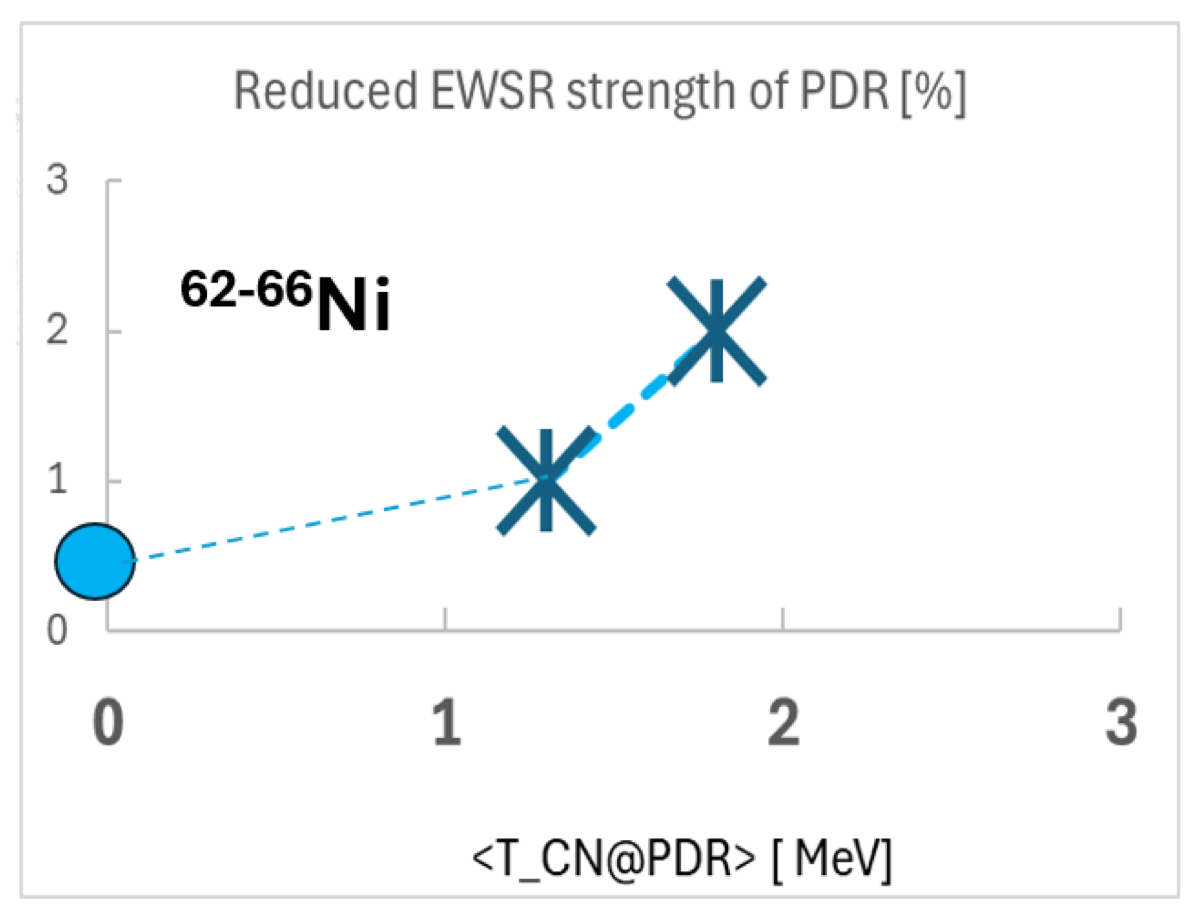
\includegraphics[width=0.6\linewidth]{graphics/Wieland.png}
    \caption{Combined preliminary results of the experiments done at CCB (circle) and IFIN (crosses). The plot shows the extra yield below the GDR for different Ni isotopes as afunction of the nuclear temperature.
}
    \label{fig:Wieland}
\end{figure}


\subparagraph{Task 2.2: Radioactive Ion Beams} \mbox{}

At \textbf{GANIL-SPIRAL2} one project focused on $^{12}$Be structure in the vicinity of different cluster thresholds, such as $^4$He, $^7$He, $^8$He by searching for narrow resonances using ACTAR-TPC detector. Second project focused at indirectly quantifying $^8$Li($\alpha$,n)$^{11}$B reaction. This reaction is involved in the nucleosynthesis from the early evolutionary stage of our universe, till the starting of r-process nucleosynthesis in supernovae, collapsars and neutron star mergers. The study has been performed by understanding the compound nucleus for the reaction, the neutron-rich $^{12}$B, with the help of the resonant elastic scattering reaction $^4$He($^8$Li,$\alpha$)$^8$Li.

At \textbf{GSI/FAIR} experiments using FRS recorded a comprehensive dataset for projectile-fragmentation products (Z = 82 to 89) from $^{238}$U on a Be target, providing essential data to refine fragmentation models and support future NUSTAR experiments. ESR has been used for investigating the rare double-gamma decay mode in 0$^+$$\rightarrow$0$^+$ transitions; this study measured isolated double-photon decays in $^{72}$Ge, and compared the two-photon decay in $^{98}$Zr and $^{98}$Mo to assess whether enhanced transition rates depend on nuclear structure, and measures of de-excitation probabilities over a wide energy range in excited $^{238}$U and $^{239}$U. For the first time, simultaneous measurements of fission, gamma, and multi-neutron emission (up to three neutrons) were achieved in a storage ring setting. R3B setup has been used for commissioning of key detectors (CALIFA, Si-tracker FOOT, NeuLAND). Cross-section measurements for (p,pd) reactions on various carbon isotopes were performed indicating the presence of strongly correlated neutron-proton pairs, with quasi-deuteron behavior influencing nucleon “dressing” in the nuclear medium. DESPEC gathered spectroscopic data around N=126 shell closer, a critical region for r-process nucleosynthesis, where new level schemes and transition probabilities help benchmark models describing the interplay of single-particle orbitals and collective excitations in heavy nuclei relevant for the astrophysical sites. FRS Ion Catcher has been used in three different experiments. A proof-of-principle study using slowed-down uranium beams in a Cryogenic Stopping Cell demonstrated that multi-nucleon transfer (MNT) reactions can produce neutron-rich isotopes (A $\approx$ 160–250). MNT products were successfully extracted and identified with the MR-TOF mass spectrometer, paving the way for future RIB production at Super-FRS (cf. \url{https://doi.org/10.1016/j.nuclphysa.2025.123041}). Also focusing on exotic nuclei from Br to Rh, this study addresses issues such as isospin symmetry breaking, the Wigner effect, and unexpected mass discrepancies (e.g., $^{70}$Br). The FRS Ion Catcher, combined with a $^{107}$Ag fragmentation beam and SIS-18 accelerator mode, delivered precise mass measurements, essential for validating nuclear models and rp-process calculations. EXPERT detector, using a $^9$C beam, probes Thomas-Ehrman shifts in mirror pairs (e.g., $^5$H-$^5$Be, $^6$H-$^5$B, $^7$H-$^7$C) and measures decay energies, widths, and half-lives (down to picoseconds) via multi-particle angular correlations. Upgraded high-rate tracking detectors have enabled high-statistics data collection, allowing for improved measurements of nuclear state widths and the identification of novel multi-proton decay mechanisms.

At \textbf{JYFL}, by using a new beta detector at IGISOL made at NCNR (Swierk/Poland), trap-assisted decay spectroscopy of very neutron-rich Rh and Pd isotopes has been performed. An interesting experiment used a reaction of deuterons on $^{242}$Pu target(s), with the goal of producing both ground states and fission isomers in $^{240,242}$Am. Set of silicon detectors were installed in the switchyard, to be used for measuring alpha activity as well as fission fragments from the decay of the isomeric states. Operated in a “duty cycle mode”, with activity monitored in the switchyard as well as beam injected into the RF cooler, either for the MR-TOF or for JYFLTRAP. The latter allowed for separation of $^{242}$Am from the target $^{242}$Pu material. Half-lives were measured, total kinetic energy of the FFs as well as the excitation energy of $^{242f}$Am with the MR-TOF. Trap-assisted decay spectroscopy of fission fragments has been performed using a beta detector connected to a tape station and surrounded by a coaxial Ge and two large BeGe detectors. This setup allowed the collection of gamma-ray transitions with energy below 20 keV in A=115 isobars region. Another project focused on neutron-deficient Ag isotopes using collinear laser spectroscopy to provide a comprehensive data set that can be used to establish a precise and accurate reference quadrupole moment for the whole Ag chain. Combined with state-of-the-art atomic calculations the aim is to investigate the consistency of quadrupole moments deduced using atomic and solid-state crystal coupling constants. A second motivation was to determine the hyperfine anomaly in Ag, which reflects changes in the distribution of nuclear magnetization. 

At \textbf{CERN/ISOLDE} several experiments addressed very topical physics in nuclei around the $^{132}$Sn double shell closure. The $^{132}$Sn(d,p) reaction has underpinned the scientific cases of many different radioactive ion beam facilities, but only a single measurement existed from more than 15 years ago before a recent ISOLDE study. This experiment studied the reaction with around ten times the intensity of $^{132}$Sn, with a higher beam energy, and with a novel spectrometer giving much improved resolution. This revealed population of $all$ the valence single-neutron orbitals for the first time and their single-particle content has been deduced, establishing them all as carrying “full” single-particle strength. In parallel, $\beta$-delayed neutron decay studies at ISOLDE have also populated the 13/2$^+$ state, with even higher energy resolution. These data on a “simple”, but exotic, nuclear system will be very impactful as they can be used in shell-model calculations of wide regions of medium-mass nuclei. The collectivity of states in this region has also been probed in Coulomb-excitation measurements of $^{130}$Sn during this period. Also using post-accelerated beams, the reaction $^{61}$Ga(d,p) was used to populate the mirror nucleus of $^{62}$Zn, an important nucleus for the astrophysical rp-process. Mirror energy differences for high-spin states in the sdpf shell were probed in a measurement of $^{39}$K(d,p) and a search was made for rotational bands at high excitation with the same beam using a $^7$Be beam. On the low-energy side of the facility, studies of laser spectroscopy have continued with measurements across many chains of nuclides, including Mg, Ca, Sb, Lu, Tm, Au and Hg isotopes. The measurements of the hyperfine structure of neutron-rich Ca isotopes are of note, shedding light on the nature of exotic shell closures and performed using a new technique that allows measurements of isotopes produced at intensities as low as 1 ion per second. Similarly, laser spectroscopy of Mg isotopes, which probed the island of inversion, demonstrated another successful new technique where ions were trapped in a mass-resolving time-of-flight spectrometer, allowing improvement in sensitivity as the laser light can probe the same nucleus very many times. Work on radioactive molecules was continued by several experimental runs, including studies of electron photo-detachment from RaF$^-$. A high statistics run was performed on the WiSARD experiment looking at non-standard model currents in weak decays using $\beta$-delayed proton emitters. Nuclear techniques were employed to characterise a number of novel materials, which included perovskites that are potentially important for novel solar cells, vanadium-based materials that have important applications in batteries, indium-gallium nitride semi-conductors, quantum colour centers in diamond that may have application as q-bits, ferroic systems such as lithium niobate that is important in piezo-electrics, and other functional materials.

Main highlights achieved by user groups in the Task 2.2 were following:

%Several experiments addressed very topical physics in nuclei around the $^{132}$Sn double shell closure 
At CERN/ISOLDE the $^{132}$Sn(d,p) reaction has underpinned the scientific cases of many different radioactive ion beam facilities, but only a single measurement existed from more than 15 years ago before a recent ISOLDE study. This experiment studied the reaction with around ten times the intensity of $^{132}$Sn, with a higher beam energy, and with a novel spectrometer giving much improved resolution. This revealed, for the first time, \textbf{population of all the valence single-neutron orbitals and their single-particle content}, establishing them all as carrying “full” single-particle strength (cf. Fig.~\ref{fig:ISOLDE_Highlight_1}). 

\begin{figure}[!h]
    \centering
    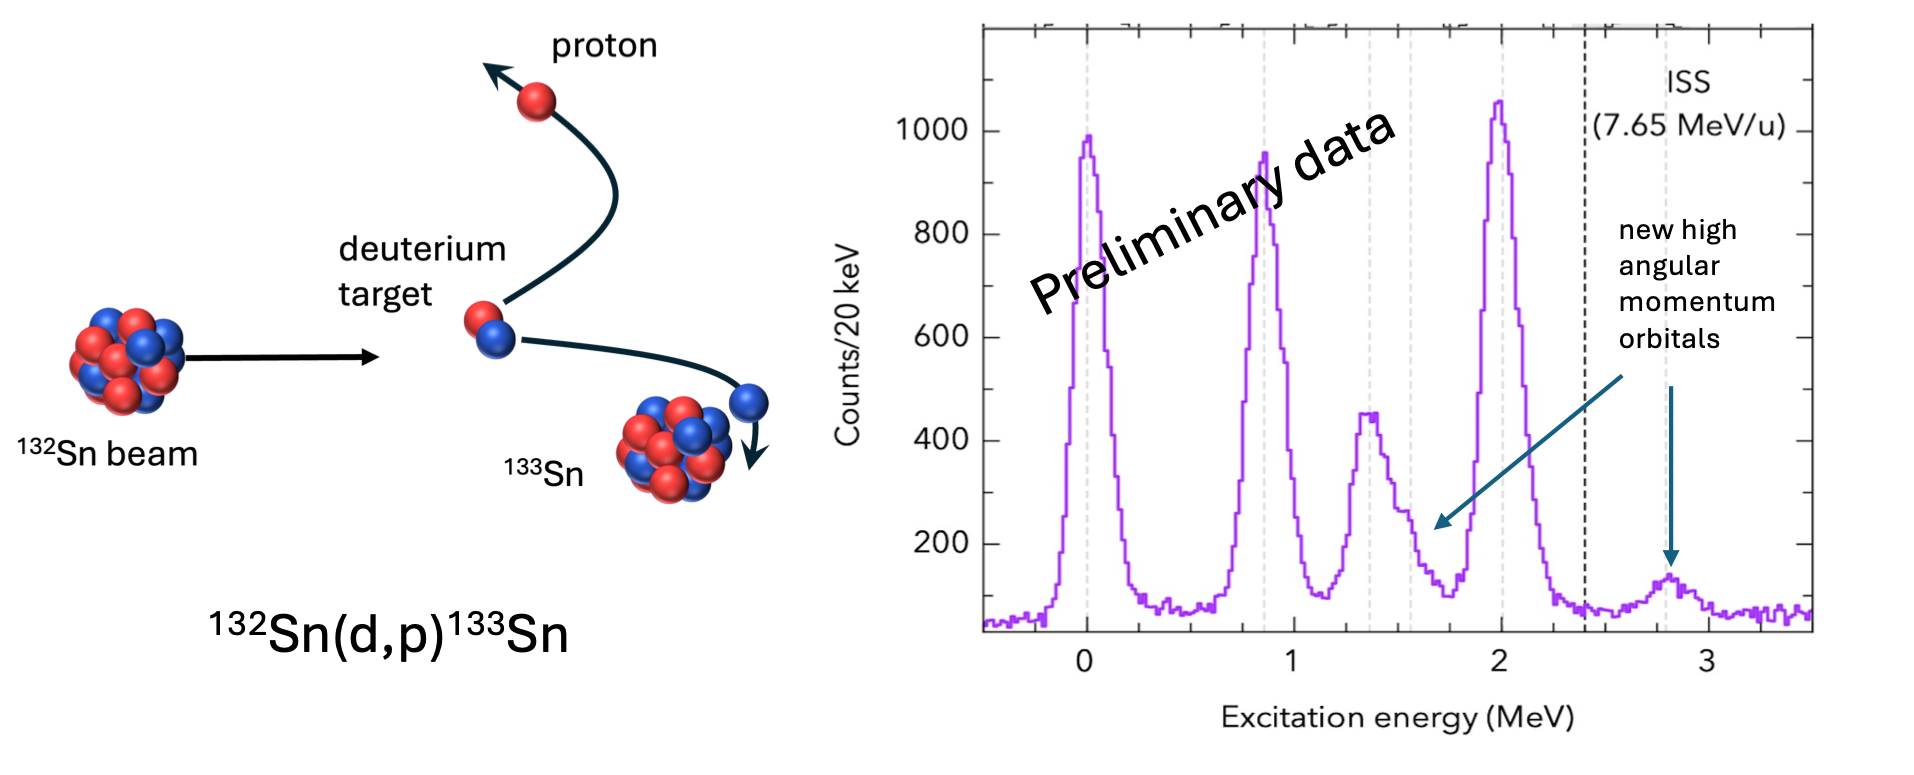
\includegraphics[width=0.9\linewidth]{graphics/ISOLDE_highlight_1.png}
    \caption{Left: A cartoon showing the mechanism for a direct (d,p) reaction.
Right: A preliminary excitation spectrum for $^{133}$Sn showing peaks corresponding to the single-neutron states outside the N=132 core.
}
    \label{fig:ISOLDE_Highlight_1}
\end{figure}

Another project at GANIL/SPIRAL2 studied the \textbf{$^{12}$Be structure in the vicinity of different cluster thresholds}, such as $^4$He and $^8$He clusters using ACTAR-TPC detector (see Fig.~\ref{fig:2alpha_cluster}). 

\begin{figure}[!h]
    \centering
    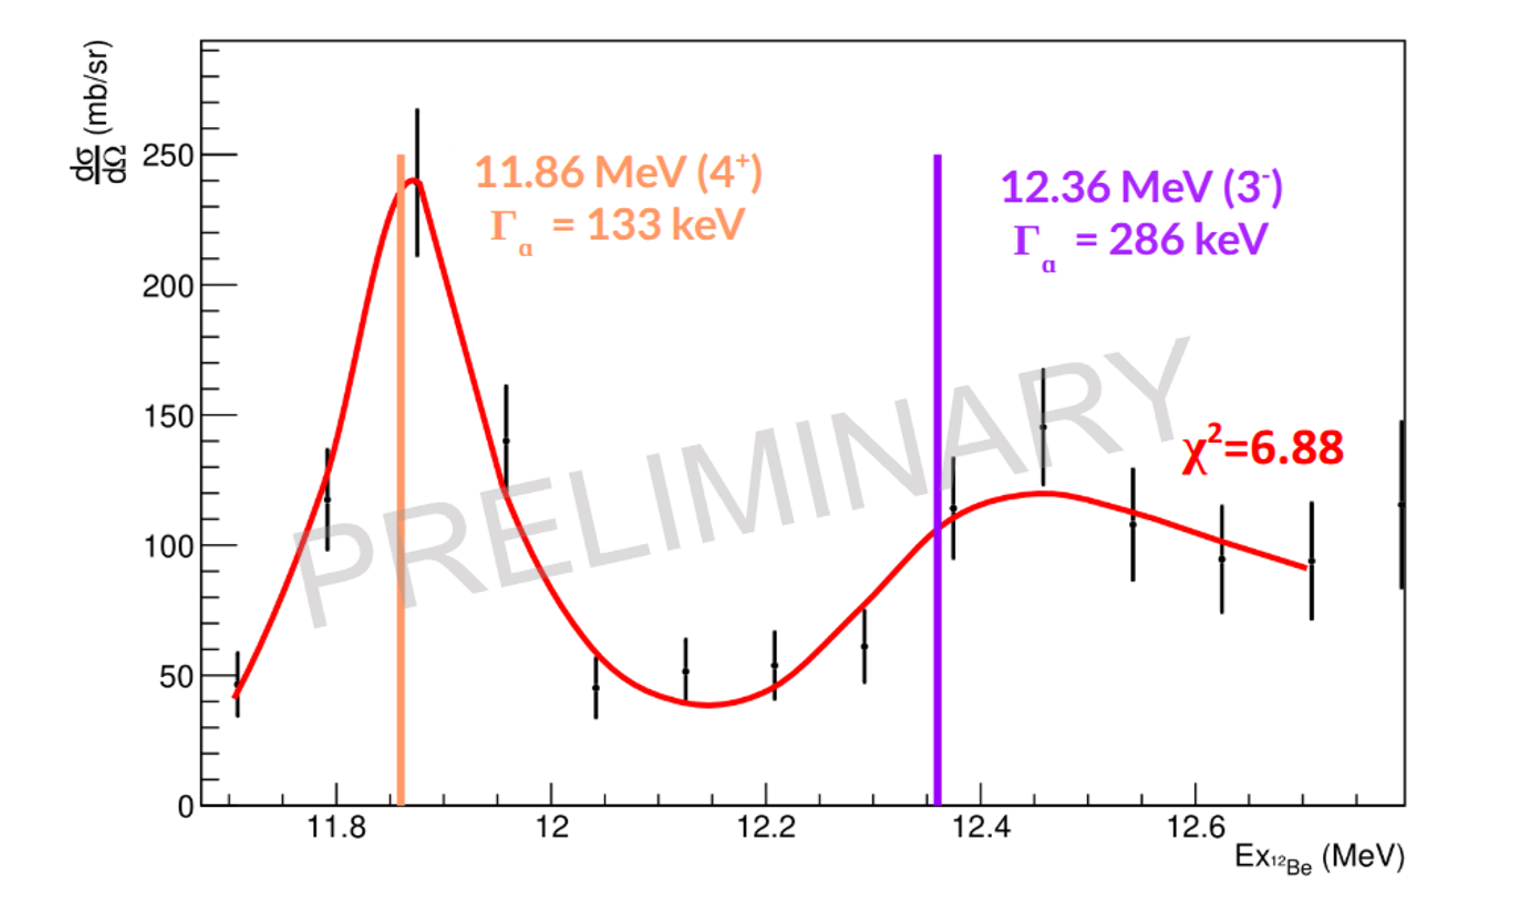
\includegraphics[width=0.6\linewidth]{graphics/2alpha_cluster.png}
    \caption{Two alpha cluster structure observed in $^{12}$Be by observing resonances in the resonance elastic scattering reaction $^4$He($^8$He,$\alpha$)$^8$He.The dark dots represents the experimental results, the red curve shows the quality of the theoretical decomposition of the results, while the violet and orange lines show the position of the cluster structure in $^{12}$Be.
}
    \label{fig:2alpha_cluster}
\end{figure}

In the project studied at JYFL joined a large collaboration from Spain (Valencia) and France (Subatech) at beta spectrometer after JYFLTRAP. This beta spectrometer has been used to directly measure the \textbf{shape of the beta spectrum of several fission fragments}. The motivation is connected to how well we understand the measured antineutrino spectrum from reactors.
%This was an excellent beam time, following on from an earlier run in 2022. Experimental improvements meant that the yields as well as the overall transmission (between 25-60\%) from the switchyard to the beta spectrometer were excellent. 
In total, around 14 cases of interest (including references) were measured, with 1 TB of data collected. These data will be sufficient to satisfy the needs of a large number of doctoral researchers in the near future.


\subparagraph{Task 2.3: Neutron Beams} \mbox{}

At the \textbf{n\_TOF} in CERN one project explored \textbf{new fission modes in lighter nuclear systems}, particularly cerium isotopes around atomic number 60 (Neodymium). Three other projects concentrated on neutron capture cross-section measurements for isotopes of Erbium and Neodymium (see Fig.~\ref{fig:n_TOF-146Nd})  improving accuracy in existing data. One of them specifically aimed to measure the $^{238}$U(n,$\gamma$) cross-section. Additionally, two projects investigated innovative techniques: measured neutron fluence using diamond detectors and testing the performances of a mixed array of HPGe and LaBr$_3$(Ce) detectors in beam.


\begin{figure}[!h]
    \centering
    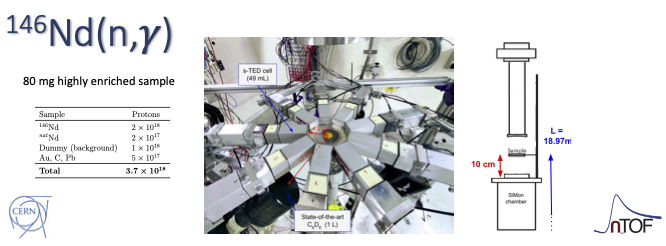
\includegraphics[width=1.0\linewidth]{graphics/n_TOF-146Nd.png}
    \caption{s-TED detector setup used at n\_TOF for the $^{146}$Nd(n,$\gamma$) reaction cross section measurement, one of the seven TA experiments executed with the EURO-LABS project support.}
    \label{fig:n_TOF-146Nd}
\end{figure}

In \textbf{CLEAR-CNA} a notable experiment was performed, measuring actinides in Baltic seaweed, characterizing novel targets for astrophysics, and assessing the impact of radioactivity from nuclear facilities. 

At the \textbf{ALTO} facility, one LICORNE project refined fast neutron tomography techniques and studied radiation damage in LaBr$_{3}$ crystals under high neutron fluence, crucial for the NUMEN project. 

At \textbf{GANIL}'s NFS facility, two key experiments investigated gas production in chromium and copper, respectively. Both projects utilized advanced experimental setups to measure double-differential cross sections for neutron-induced reactions, contributing valuable data for future fusion plant simulations and nuclear reaction models.

\subparagraph{Task 2.4: Theoretical Support} \mbox{}

The theoretical support offered at \textbf{ECT*} covered a broad range of subjects in various workshops, which were characterized by a high degree of interaction and collaboration among participants. At a fundamental level, progress has been achieved in the theoretical description of how quarks and gluons interact to give rise to the nuclear forces that shape the structure of nuclei. Strategies were mapped out to probe generalized parton distributions through novel exclusive processes and to use Lee-Yang singularities to determine the critical point of the QCD deconfinement transition. It was clarified that while global equilibrium in the QCD plasma probed in heavy-ion reactions is unique and independent of the pseudo-gauge choice, the definition of local equilibrium differs in quantum kinetic theory and quantum statistical field theory and is furthermore susceptible to a pseudo-gauge ambiguity. New directions have been charted for an {\it ab initio} development of optical potentials, including the Dispersive Optical Model and Green’s Function Theory, which are essential for the extraction of nuclear properties from lower-energy reactions. The takeaways for stellar dynamics, sensitivity studies, and astrophysical observations (including the determination of elemental abundances in stars) were extracted from key astrophysical reactions studied at facilities such as LUNA (Italy), JUNA and LEAF (China), CASPAR (USA), STELLA (France), Felsenkeller (Germany), and various large RIB installations. A Doctoral Training Program further enhanced the training of early career researchers in nuclear astrophysics, in particular the interplay between theory, experiment, and observations in the determination of the neutron-matter equation of state, as well as its impact on the neutron-star dynamics, neutrino emission, nucleosynthesis, and (gravitational and electromagnetic) signals from mergers. A separate workshop probed the extent to which these signals could provide a smoking gun for the presence of hyperons in neutron stars, which is strongly influenced by two- and three-body hyperon-nucleon forces inferred from information on hypernuclei. Nuclear theorists informed experimentalists of the specific data that is needed to benchmark and further develop models for neutrino-nucleus interactions, as needed for the analysis of next-generation oscillation experiments. Novel opportunities were identified for the determination of electric dipole moments, a sensitive probe of physics beyond the Standard Model of particle physics, such as a radioactive isotope/molecule program that could be envisioned at PSI (Switzerland). The nuclear physics opportunities of new high-power laser facilities, such as ELI-NP (Romania) have also been explored. Discussions on modern algorithms in machine learning and data analysis (from medical physics to research with accelerators and in underground laboratories) identified generative models at the LHC (Switzerland) as a promising strategy to reduce computing time, though challenges in deployment were acknowledged.

Overall, all of these initiatives of WP2 highlight significant advancements in nuclear physics research and the importance of collaborative efforts between theorists and experimentalists across various facilities.
%
% 
\subparagraph{Work Package 3 - Access to RIs for Accelerators} \mbox{}
\label{sec:wp3_scientific_output}
% \todo{Scientific output of WP.}


The scientific projects conducted by the WP3 TA users span a wide range of research frontiers, benefiting from the unique capabilities of the facilities. Some highlights are presented below.

\textbf{\textit{Laboratory Astrophysics}} \mbox{}

The \textbf{HRMT-62} and \textbf{HRMT-64} series of experiments, conducted during P2 at the HiRadMat Facility at CERN, focuses on pioneering and high-quality R\&D utilizing the unique characteristics of the facility to conduct laboratory experiments for astroparticle research. The HRMT-62 experiment inaugurated and demonstrated the use of the HiRadMat facility to produce high-intensity, high-density, ultra-relativistic, quasi-neutral electron-positron pair beams, thereby opening up the possibility of studying the microphysics of such pair plasmas through experimental means.
In the subsequent HRMT-64 experiment, with an improved setup that included a secondary target and a magnetic collimating system, the focus was on studying the emergence of magnetic fields associated with the growth of filamentation instabilities. This was done by observing the propagation of collimated relativistic pair-plasma beams through ambient plasma, an analogue for the propagation of astrophysical pair jets through the intergalactic medium.

The results of the experiments were published in well known scientific journals with high impact, triggering the attention of hte community. Up to-date, 5 peer-reviewed articles have been written, 3 of them published in or submitted to Nature, all citing the EURO-LAB support. In total, 14 press releases have been done by the collaborating institutes, including 2 from CERN (bulletin \& courrier). It worth noting that the articles have a high ``attention score'', of 260: 99th percentile of the 329,972 tracked articles of a similar age in all journals. The key scientific result from HRMT-64, only made possible with the EURO-LABS support, was the first-time measurement of the magnetic fields produced by plasma instabilities using a Faraday rotation, seen in Figure~\ref{fig:hiradmat_mag_field_plasma}.
\begin{figure}[H]
    \centering
    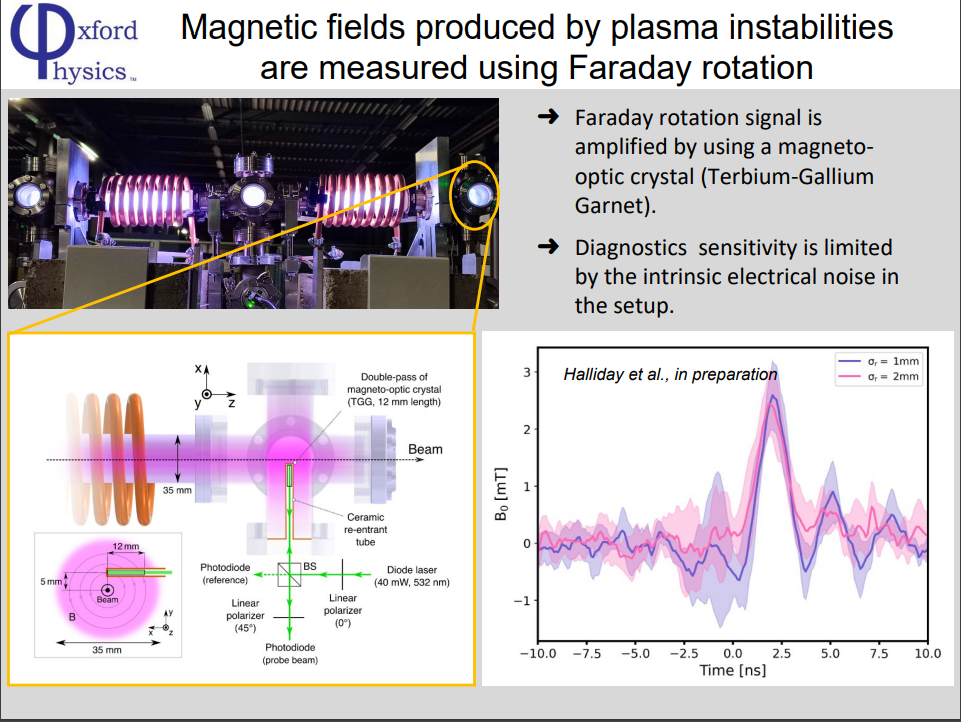
\includegraphics[width=0.75\linewidth]{graphics/HRMT_64_magnetic_field.png}
    \caption{HRMT-64, with the EURO-LABS support measured for first time the magnetic fields produced by plasma instabilities using a faraday rotation in HiRadMat. Courtesy: Prof. G. Gregori, Univ. of Oxford.}
    \label{fig:hiradmat_mag_field_plasma}
\end{figure}

\textbf{\textit{Material R\&D}} \mbox{}

\textbf{HRMT-66} was a novel experiment that pushed forward our current knowledge of material limits, particularly for the often used Glassy Carbon and Beryllium, along with a first-time irradiation of Si$_{3}$N$_{4}$ in order to investigate its exact damage threshold. This is very important for the cooling section of a future muon collider. A photo from the results is shown in Figure~\ref{fig:hiradmat_Si3N4} for Si$_{3}$N$_{4}$ and in Figure~\ref{fig:hiradmat_GC} for Glassy Carbon. The support of EURO-LABS was extremely important since FLUKA simulations were absolutely necessary for the evaluation of the damage mechanisms and precence at CERN was vital for some of the collaborators of the experiment.

\begin{figure}[!h]
    \centering
    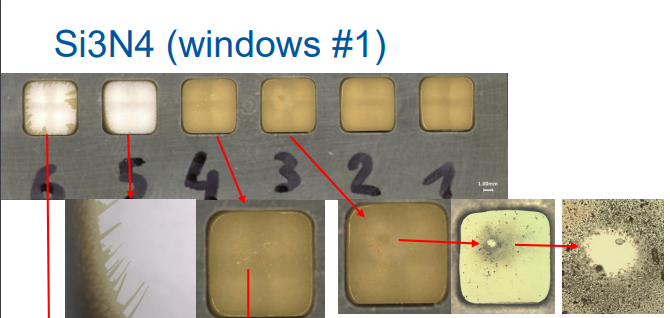
\includegraphics[width=0.85\linewidth]{graphics/hiradmat_si3n4.png} \\
    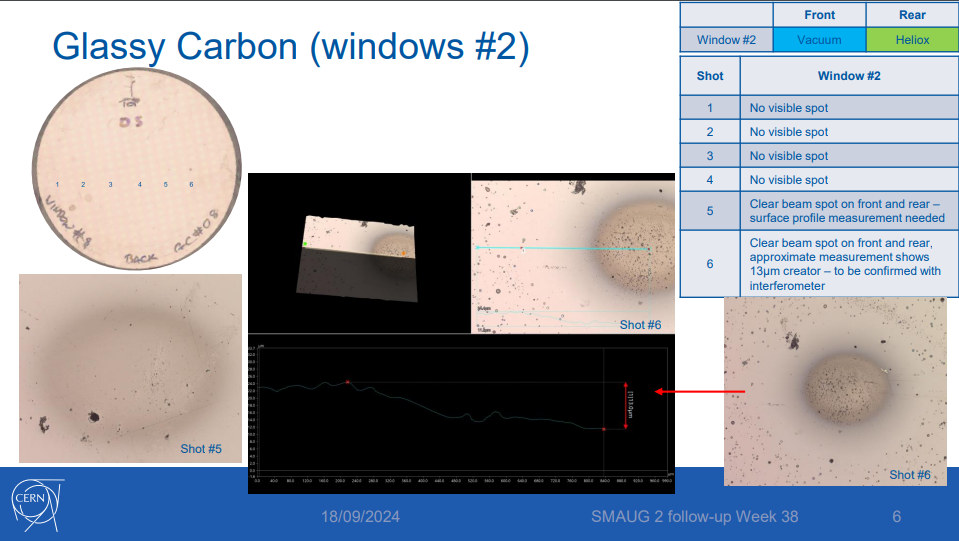
\includegraphics[width=0.85\linewidth]{graphics/hiradmat_GC.png}

    \caption{Top : Beam impact on Si3N4 windows during HRMT-66 experiment. The clear beam spot can be seen in shot \#6 including a small crater. Bottom : Results from HRMT-66 experiment on Glassy Carbon. . (Courtesy: A. Harrison, CERN)}
    \label{fig:hiradmat_Si3N4}
\end{figure}


\textbf{\textit{Instrumentation R\&D}} \mbox{}
\textbf{HRMT-55} is a collaboration between CERN and ESS, to develop a new generation of ionization chambers able to work in high intensify environments, of interest for both Organizations.

Figure~~\ref{fig:hiradmat_IC_response} shows the response of different ionisation chambers (IC) tested for increasing beam intensity. The results indicate a close-to-linear detector performance for all , however with large variations in slope between them. 
\begin{figure}[!h]
    \centering
    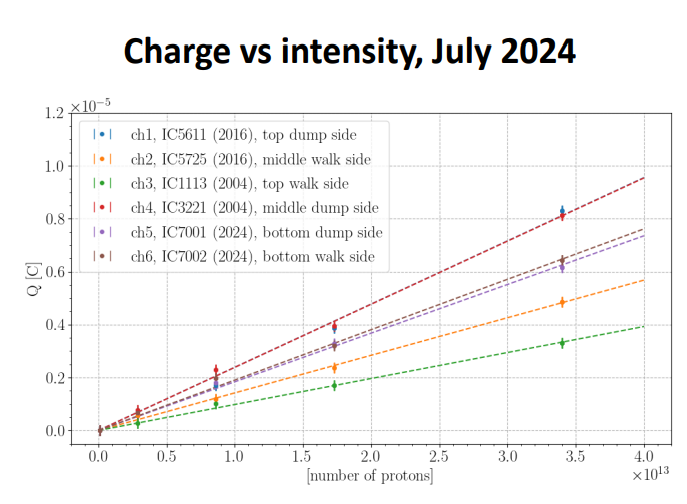
\includegraphics[width=0.8\linewidth]{graphics/hiradmat_IC_response.png}
    \caption{Response (C) of the different ionization chambers tested in HRMT-55. The difference in the slope needs to be understood in detail in a follow-up experiment (HRMT-71) planned for 2025. (Courtesy. S. Grishin, ESS)}
    \label{fig:hiradmat_IC_response}
\end{figure}
This is, for the moment, a puzzling result; therefore, a follow-up experiment \textbf{HRMT-71} is planned for 2025 to further investigate the underlying reasons.

\textbf{R\&D for future accelerators - I}
\todo{PIP-II cavities in SUPRATECH-MACHAFILM}

\textbf{\textit{R\&D for future accelerators}} \mbox{}

Particle accelerators and colliders must cope with a large amount of synchrotron radiation (SR) power being deposited on the vacuum chamber walls.
Photo-stimulated desorption (PSD) leads to increasing pressure and high heat load and is therefore to be investigated using new types of a number of beam screen and vacuum chamber prototypes. The results of this study will be critical for the design of future high-energy hadron colliders such as FCC-hh, in addition this research has potential implications also for the near future of the LHC. 
\begin{figure}[H]
  \centering
  \begin{minipage}[c]{0.45\textwidth}
    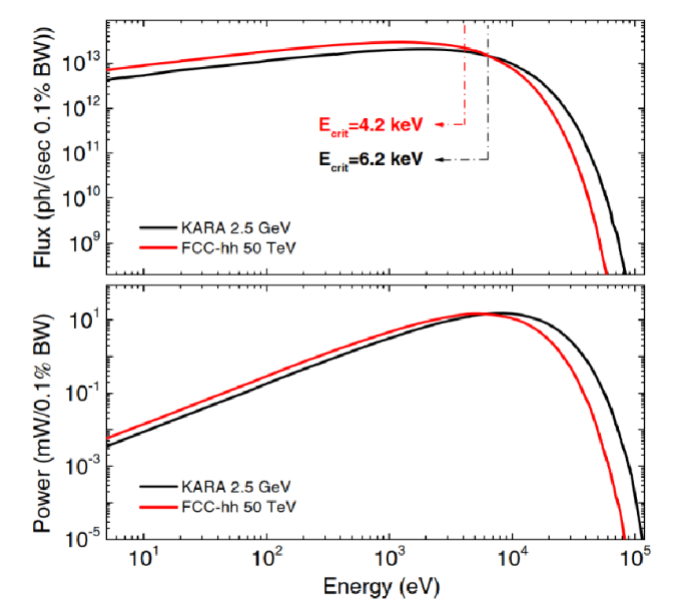
\includegraphics[width=\textwidth]{graphics/wp3-KIT_FCCphotons.png}
  \end{minipage}%
  \hfill
  \begin{minipage}[c]{0.5\textwidth}
    \vspace*{\fill}
    \captionof{figure}{Comparison of the photon flux (top) and power (below) of the FCC-hh at \SI{50}{TeV} proton beam energy in comparison with KARA's at its nominal \SI{2.5}{GeV} electron energy for user %operation. Calculations were performed with SYNRAD+~\footnote{see: L. A. González et al. DOI: 10.1103/Phys.Rev.Accel.Beams 22, 083201, and L. A. González et al. (2021) Phys.Rev.Accel.Beams 24, 113201}
    }
    \label{fig:yourlabel}
    \vspace*{\fill}
  \end{minipage}
\end{figure}

During the EU-project EuroCirCol CERN and KIT realized the BESTEX beamline of CERN at the KIT light source. The storage ring of the KIT light Source is the synchrotron KARA delivering similar spectra as expected at the FCC.

CERN installed a residual gas analyser in the central part of the BESTEX test chamber  before the start of the FCC beam screen prototype experiment (no.5, with saw-tooth profile to decrease synchrotron radiation photon scattering) in period P1 (EURO-LABS-KIT-KARA-2023-01). In period P2 this prototype was exchanged by the new beam-screen prototype no. 6 with amorphous carbon coating (aC). aC is a stable and inert material, deposited via sputtering techniques onto the internal wall of a circular tube (carried out at CERN).  The main feature of aC is its extremely low secondary electron yield, which is necessary to avoid electron cloud instability in accelerators with positively charged beams. In the long-term experiment at KARA (EURO-LABS-KIT-KARA-2023-03), the beam-screen prototype no. 6 was irradiated at a flat angle of incidence and cooled with LN2. The increase in pressure was measured. In addition, the composition of the species outgassing from the beam screen was determined at CERN's BESTEX beamline at KARA. The experiment began installation in August 2023 and the prototype was irradiated with over 480 KARA synchrotron light until the first quarter of 2024. The prototype is still installed in BESTEX and is waiting to be exchanged for the next one, which is currently being prepared
\begin{figure}[!h]
    \centering
    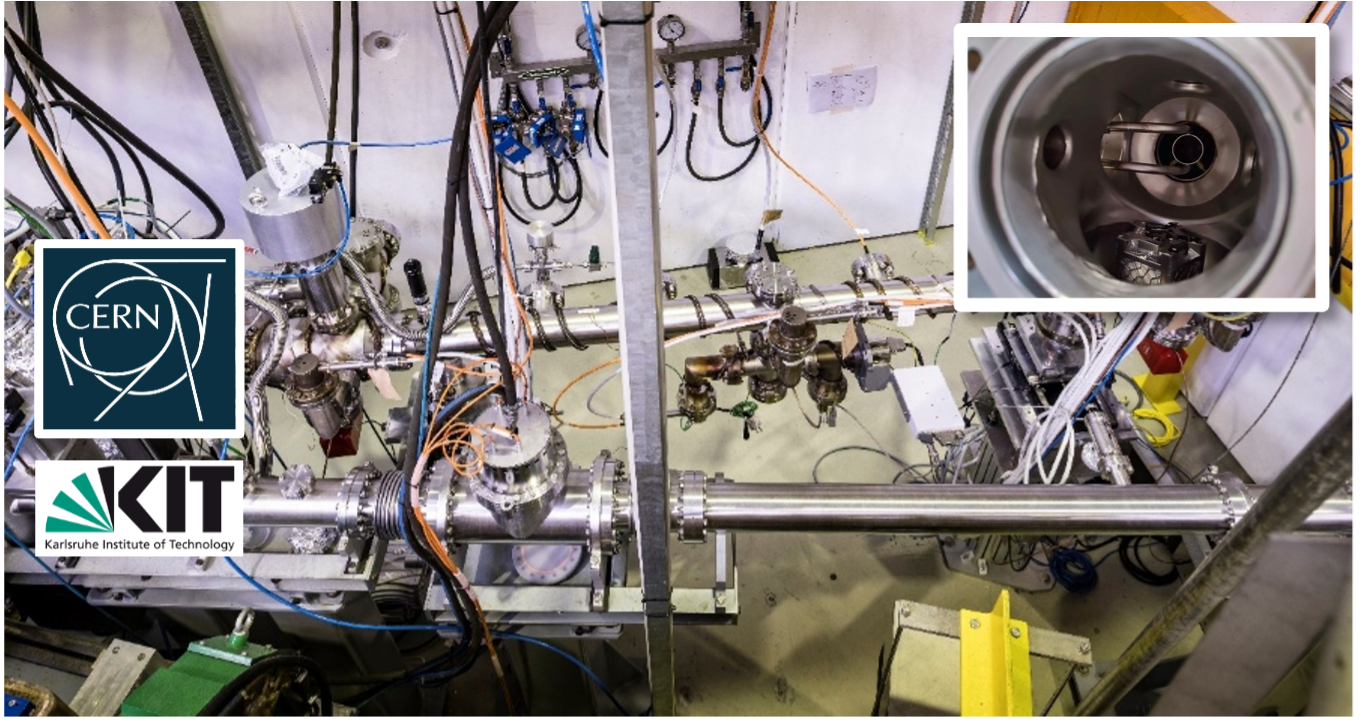
\includegraphics[width=0.75\linewidth]{graphics/wp3-KIT_BESTEX.png}
    \caption{CERN installed the BESTEX beamline at KARA since 2019 (EU project EuroCirCol). BESTEX was used for up to now two actual TA experiments within EURO-LABS. A goal is the exploration of the vacuum performance of the FCC-hh beam screen to protect the cold superconducting magnets from the 
direct irradiation high-power SR photon beams.
}    
    \label{fig:kit_bestex}
\end{figure}

The KARA experiment (EURO-LABS-KIT-KARA-2023-04) of the University Lille aimed to observe, understand and control the ultrafast self-organisation of relativistic electron bunches in accelerator facilities. A central goal is to master the emission of giant terahertz (THz) pulses in coherent synchrotron radiation (CSR), which is a proposal for new THz sources. Another important goal was the improvement of novel ultrafast observation instruments. KARA is one of the only electron storage rings in the world where the shape of relativistic electron bunches can be directly ‘studied’ in a storage ring facility. The techniques of chaos control (feedback control of periodic orbits) for achieving stable THz-CSR emissions, which the team at the University of Lille had already successfully tested at the SOLEIL synchrotron, were transferred to the KIT light source KARA, and the results have thus been compared between the machines and with theory. At KARA, the opportunity was taken to observe the development of the longitudinal bunch profile in real time with the help of the existing electro-optical near-field setup. In this experiment, an advanced control loop from chaos control theory was implemented on a fast FPGA board to control the amplitude of one of the two main radiofrequency (RF) cavities in the electron storage ring KARA at KIT. The CSR emission of THz power at high level was stabilised to control the micro-bunching instability. The fast Schottky diodes in the KIT-IR2 beamline at KARA were used and the THz power was measured in real time with the high-speed data acquisition card KAPTURE developed by KIT.
\begin{figure}[H]
    \centering
    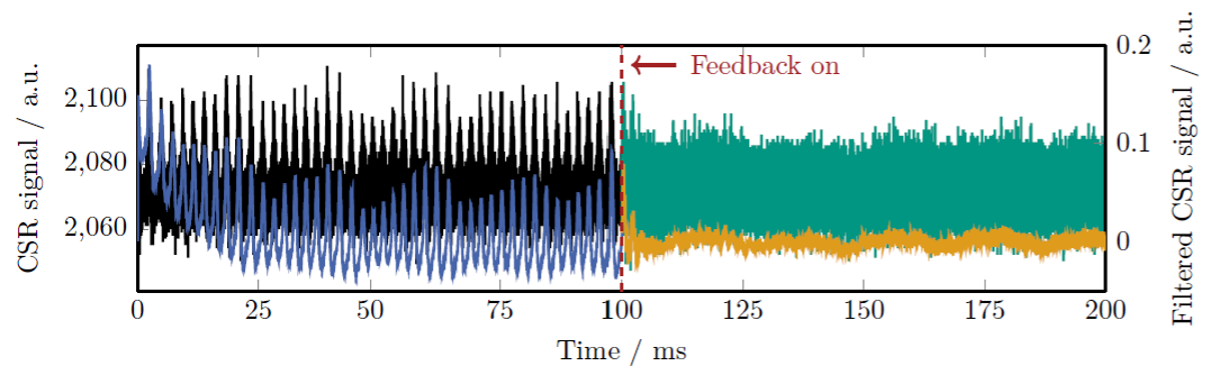
\includegraphics[width=0.75\linewidth]{graphics/wp3-KIT_CSRsignal.png}
    \caption{The CSR signal was measured with a fast Schottky diode (at a KIT infrared beam line). After \SI{100}{ms} the team of the University Lille (F) switched on the FPGA-based feedback loop. For better visibility, the raw signal (black, left \& green, right) was filtered (blue, left \& orange, right) to remove the fast sinusoidal fluctuation. Suppression of the sawtooth outburst fluctuation variance by a factor of 28 in the CSR emission at the KARA electron storage ring, after switching on the FPGA-based feedback loop developed by the PhLAM team of University Lille. The fast CSR fluctuations are still present after the feedback is switched on, leading to a stabilization of the THz emission. Publication in preparation.}    
    \label{fig:kit_csr}
\end{figure}

FCC-ee precision physics measurements require an accurate and precise determination of the centre-of-mass collision energy, which can be obtained from the beam energies. Since the depolarisation frequency is directly proportional to the beam energy, a promising way to determine this energy is to depolarise transversely polarised packets. This resonant depolarisation (RDP) has long been used in KARA whereby the resonance frequency is measured via the change in the Touschek lifetime. At KARA, a first RDP measurement campaign (EURO-LABS-KIT-KARA-2023-05) with numerous scan settings and bundle configurations was carried out to investigate how this technique could be applied at FCC-ee, in particular the sensitivity to parameters such as the scan speed of the depolariser and the scan velocity. The measurement campaign was successful and the users at CERN expressed interest in carrying out another measurement campaign at a later target point.
\begin{figure}[H]
    \centering
    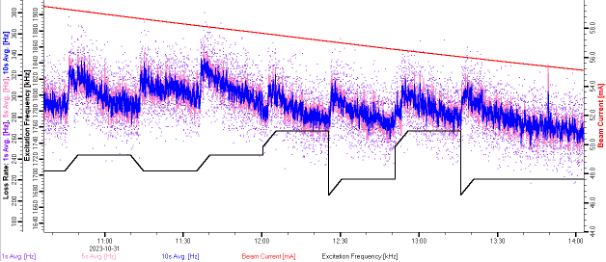
\includegraphics[width=0.75\linewidth]{graphics/wp3-KIT_RDPscans.png}
    \caption{More than 40 successful RDP scans were realized at KARA by scanning direction up and down for scanning times of \SI{100}{s} to \SI{600}{s}, respectively}    
    \label{fig:kit_rdp}
\end{figure}

RDP results published in:
\begin{itemize}
\item FCCIS WP2-workshop, 2023-11-15, B. Härer et al.: Polarisation studies at KARA
\item and in the following IPAC papers: \\ https://doi.org/10.18429/JACoW-IPAC2024-TUPG33, \\ https://doi.org/10.18429/JACoW-IPAC2024-WEPG51, and \\ https://doi.org/10.18429/JACoW-IPAC2024-WEPR20
\end{itemize}

Bunch-by-bunch (BBB) feedback systems are essential for the realisation of ultra-low emittance rings that allow electron beams to reach high-quality states for use in synchrotron radiation light sources and colliders. Following the workshop WP7.2 of the EU project I.FAST on BBB feedback systems, which was attended by more than 40 experts on BBB systems from all over the world, the following three experiments were carried out at the request of the experts in connection with the BBB systems carried out at the KARA storage ring and at the booster synchrotron with real electron beams by operating the BBB systems installed in each of the two accelerators(EURO-LABS-KIT-KARA-2024-06). The aim of the first experiment at KARA was to manipulate the vertical beam size by exciting the betatron oscillation with the BBB system to improve the Touschek beam lifetime. The goal of this experiment was to look for common procedures for commissioning bunch-by-bunch feedback systems. The goal of the third experiment was to longitudinal kicks with the bunch-by-bunch feedback system and the stripline kicker installed in the booster synchrotron. This experiment will lead to the next step, such as longitudinal manipulation of beams to improve booster beam quality. Data and results of the three experimental topics have been shared with all interested participants, and the data analysis and subsequent discussions are ongoing. 


According to the design of the FCC, the desired mechanical alignment tolerances of the magnets are in the range of \SI{100}{\micro\meter} to \SI{150}{\micro\meter}. However, to achieve the ambitious research goals at the FCC, a low (10-20 µm) relative alignment of the quadrupoles and sextupoles is required. For this purpose, correction magnets are provided to steer the beam in the direction of the magnetic centre, which is known as beam-based alignment (BBA). The BBA must be performed for approx. 1870 quadrupoles and approx. 630 sextupoles, so in addition to the accuracy, the average time required to determine the individual magnetic offset is a key parameter for the selection of the BBA method. The development of a concept for the BBA at FCC-ee is currently based on simulations but is to be supported by proof-of-principle tests on existing machines, for which experiments were carried out at KARA (EURO-LABS-KIT-2024-KARA-07).  Strategies were successfully investigated that will significantly reduce the time required for the BBA at FCC.


\textbf{\textit{Novel detector R\&D}} \mbox{}

\begin{description}
\item[MM\_TCP]: The experiment goal was to test and validate TPC performances of two MicroMegas detectors based on a strip read out system. The resistive Micromegas chambers are frontier Micro-Pattern Gas Detectors with a planar geometry and with an amplification gap of the order of \SI{18}{\micro\meter} between the read-out (RO) PCBs and the mesh. Similar detectors have been widely used and recently installed in the muon spectrometer of one of the LHC experiment, covering a dimension of \SI{2400}{\meter\tothe{2}}.
The purpose of the test beam is to study and tune the DAQ based on APV technology in order to adapt to the acquisition window required for TPC purposes.
\begin{figure}[H]
    \centering
    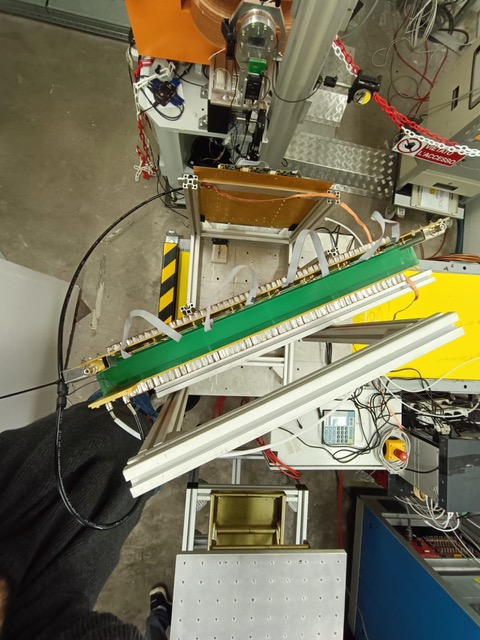
\includegraphics[width=0.48\linewidth]{graphics/BTF-MMTPC2.jpeg}
    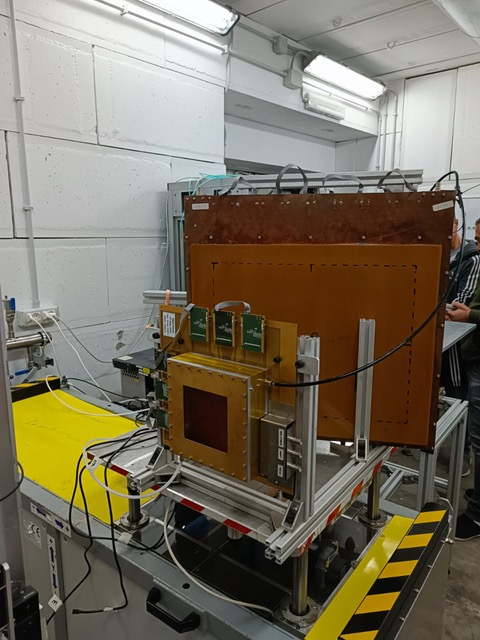
\includegraphics[width=0.48\linewidth]{graphics/BFT-MMTPC3.jpeg}
    \caption{Photo of the experimental setup in the BTF line.}    
    \label{fig:kit_rdp}
\end{figure}
Two different types of Micromegas, one of which never previously tested, have been experimentally characterized. The planned test and some other extra test have been fully acquired, with calibration and load curve in different beam configuration especially for flux and multiplicity.
The experiment resulted to be well-planned, executed smoothly, and achieved its goals. The combination of on-site and remote support, along with continuous monitoring of the system parameters, contributed to the overall success of the operation.
Experiment Duration: 1 week or 168 h (2023, 20-27 November)

\item[MICROGASTRACK]:
The experiment aimed at testing a novel micromegas gas chamber with variable high voltage which could enable both to track the secondary particles produced in the interactions and to measure the initial high intensity beam parameters. The device under test combines the functionalities of micropattern gas detectors for precise sub millimetre tracking and gas detectors for beam monitoring.

The detector that was expected to be ready for the test beam time, was unfortunately not completed in time. However, the team was able to test the MM electronics and integrate with the BTF timing and triggering. Additionally, during the beam time, a successful integration of future detector support was achieved. The team had also the possibility to test the detector electronics (APV25) and the communication with the pre-existing DAQ system
Experiment Duration: 2 weeks or 336 h (2024, 4-18 November)

\item[CALOBEAMPIX]:
The experiment goal was to test silicon pixel detectors for simultaneous measurement of electron/positron beams with two different types of detectors: calorimeter and silicon pixel detector. 

The following experimental goals were reached:
\begin{itemize}
    \item Operate simultaneously Timepix3 array and lead glass calorimer
    \item Develop threshold equalization procedure for the Timepix3 pixels
    \item Synchronized data acquisition (either online or offline) of Timepix3 and lead-glass calorimeter
    \item Calibrate the lead glass block for different beam multiplicity using the Timepix3 data
\end{itemize}
Experiment Duration: 1 week or 168 h (2024, 9-16 December)
\end{description}


%\textbf{Medical Physics R\&D}

%\begin{description}
%    \item[AI1] Artificial Intelligence readiness at CLEAR. Done, Reimbursed (A. Pollastro, 40 units)
%    \item[LUXE2] Done, reimbursed (F. Lasagni-Manghi, 40 units)
%    \item[THz] THz sources on Smith-Purcell radiation, THZ1 > Initial visit + preparation done,  will not be reimbursed (paid by Users Lab) (T. Zhang, 16 units)
%    \item[SE1] Electron collimation at CLEAR (SE1) > Done, to be reimb. (N. Delerue, D. Dauvergne, 64 units)
%\end{description}

\textbf{Applications}


\begin{itemize}
\item One-electron oxidation of S-adenosyl methionine,
\item Crosslinking of self-assembled fatty acids on copper by electron beam irradiation,
\item Effect of ionizing irradiation on dried fruits,
\item Influence of 10 MeV accelerated electrons on structure and properties of sheep wool fibres as a potential component for preparation of polymer-based composite materials
\item Irradiation engineering of biopolymer-based formulation for wound management and targeted drug delivery devices,
\item Bioactivity of irradiated foods by low energy e-beam,
\item Face masks recycling with the use of radiation technologies.
\end{itemize}
%
% 
\subparagraph{Work Package 4 - Access to RIs for Detectors} \mbox{}

WP4 is the enabler of Detector R\&D, the fundament of current and future scientific endavour. Most of its scientific output is thus hidden, displaced to the developed detectors, their implementation in experiments and the fundamental physics discoveries those experiments shall unravel. Needless to list what shall be discovered – if we knew that, there would be no need for conducting experiments.

WP4 is of vital importance for the successful completion of the HL-LHC project, the focal point of the European Strategy for Particle Physics (ESPP) in 2013 and its update in 2020. The upgrades have nearly finished their R\&D and the construction of the detectors is in full swing. There are, however, late surprises that still require verification of the solutions in the WP4 RI’s. The experiment upgrades for the LHC are amply documented in the respective Technical Design Reports (TDR) and in the Memoranda of Understanding (MoU) for the specific detectors, available on the CERN Document Server (CDS).

The shift of focus in WP4 is synchronized with the stipulations of the ECFA Detector R\&D Roadmap, serving either the medium term goals like the Higgs factory or the more distant endeavour towards the highest energy hadron collider (FCC-hh). WP4 backs up the newly set up DRD collaborations by providing them with access to top-level infrastructure needed for their detector R\&D. The more precise guideline to future facilities, e.g. which Higgs factory to build in the next decade is expected from the currently ongoing strategy process (ESPP), to be adopted by the CERN Council in early 2026.

The spectrum of DRD collaboration research activities is best illustrated in their proposals and their structuring into Work Packages and Working Groups. They follow closely the programme, set up by  the DRD Themes (DRDT) specified in the Detector R\&D Roadmap.

WP4 is delivering the services needed for detector R\&D. The resulting scientific output in terms of publications is two-fold: scientific results in instrumentation are being published in scientific journals and conference proceedings during the duration of the project. The more glorious part with the physics results of the HL-LHC experiments and their follow-ups at future colliders will, however, start emerging during the next decade and beyond, when the detectors now being tested at WP4 RIs will be put to their proper usage and deliver precious physics data.


\tsubsubsection{Virtual access (VA) activities}



The \textbf{Theo4Exp} VA facility consists of 3 installations: \textbf{MeanField4Exp} in IFJ PAN Krakow, \textbf{Reaction4Exp} in USE Sevilla, and \textbf{Structure4Exp} in U. Milano. The users can access any of the 3 installations via a common entry point \url{https://institucional.us.es/theo4exp/}. In the 2nd Reporting Period 1915 AU (counted as each started hour of active use of the virtual service) were provided to 185 users (see Fig.~\ref{fig:WP2_VA_statistics}) from 21 countries worldwide (see Fig.~\ref{fig:VA_countries}). 

\begin{figure}[!h]
    \centering
    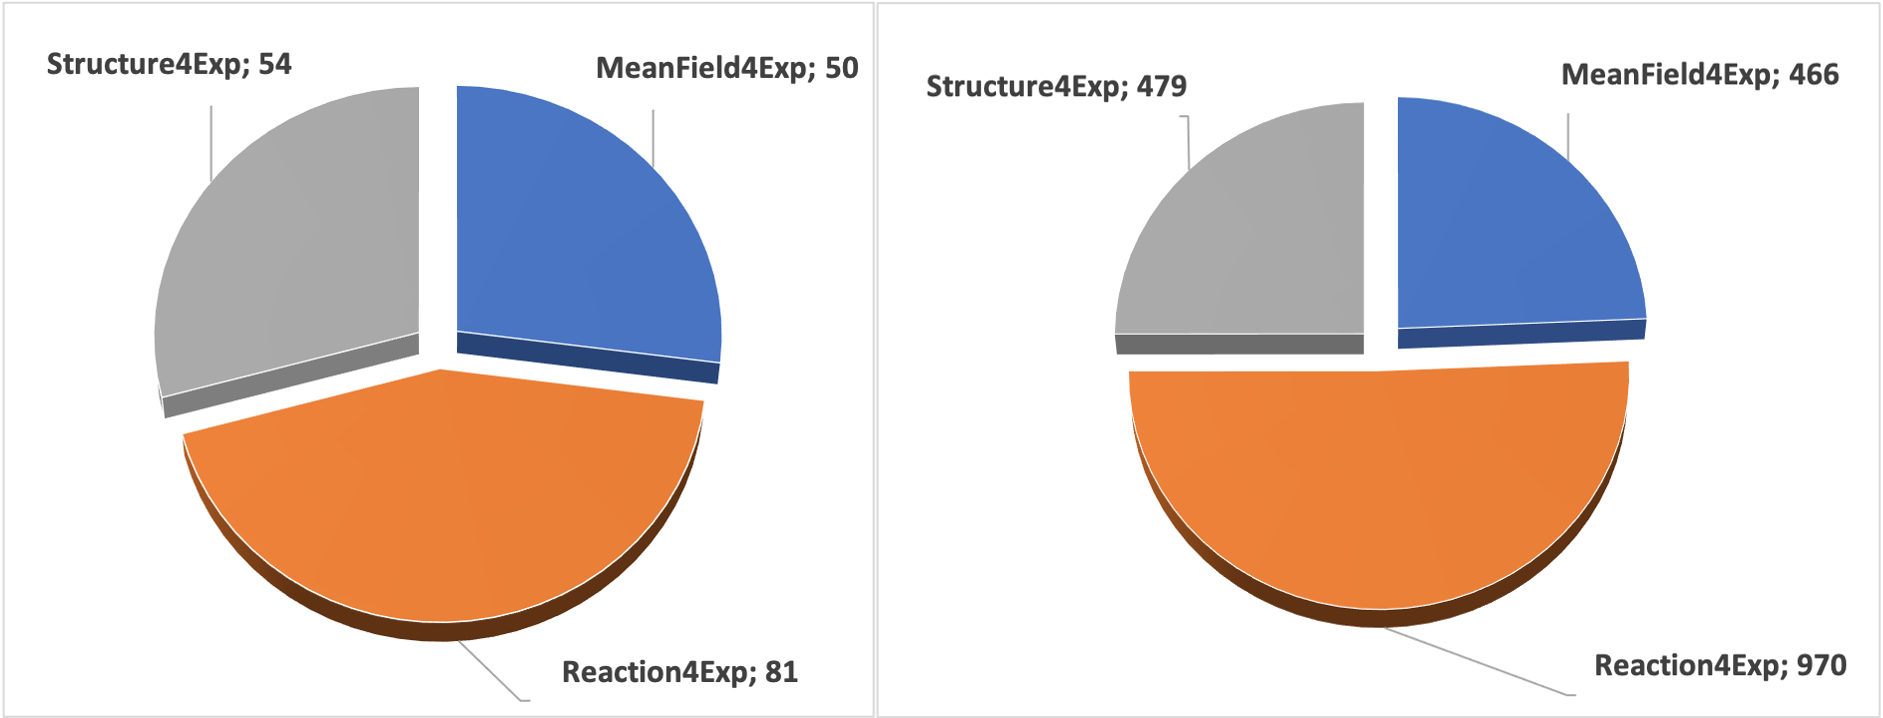
\includegraphics[width=1.0\linewidth]{graphics/WP2_VA_statistics.png}
    \caption{Distribution of users (left) and provided Access Units (right) between the Theo4Exp VA facility installations.}
    \label{fig:WP2_VA_statistics}
\end{figure}

\begin{figure}[!h]
    \centering
    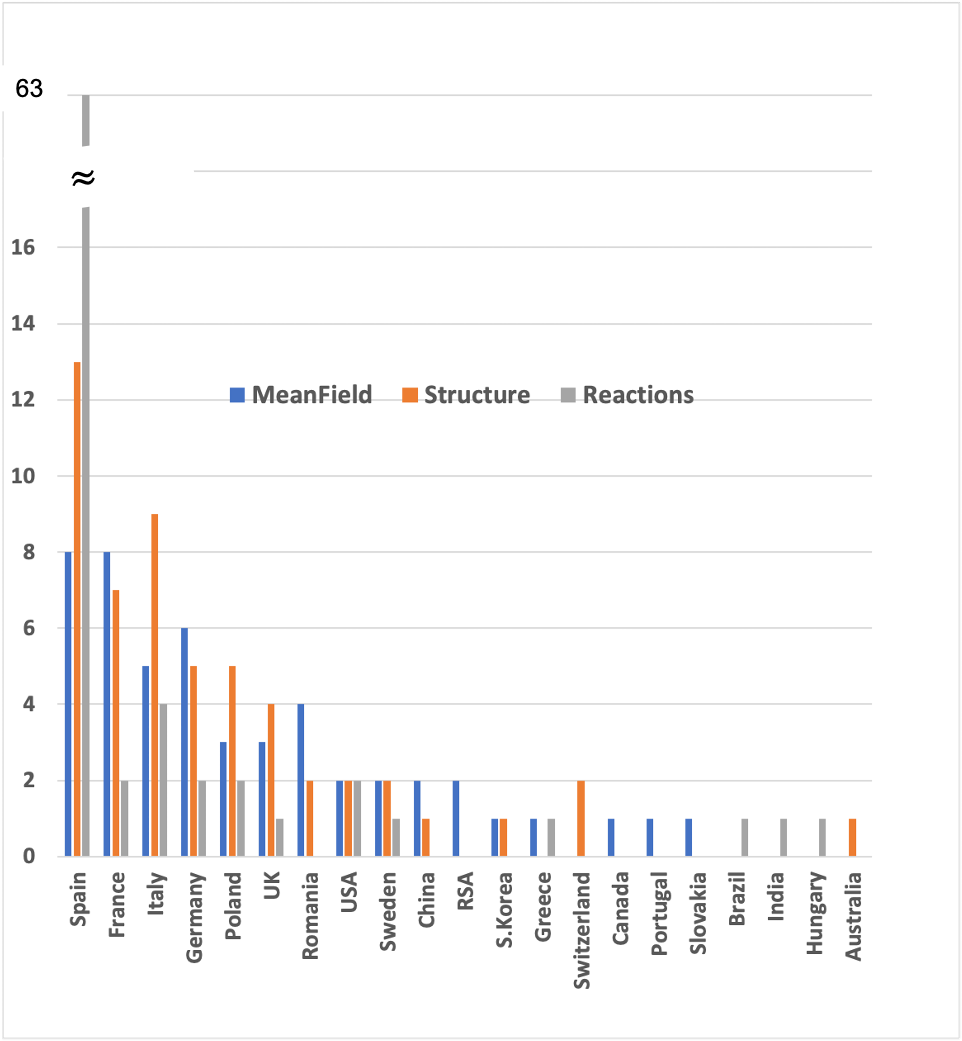
\includegraphics[width=0.85\linewidth]{graphics/VA_countries.png}
    \caption{Geographical distribution of Theo4Exp VA installations users during P2.}
    \label{fig:VA_countries}
\end{figure}
The following activities were carried out in P2 in the 3 installations:

In IFJ-PAN \textbf{MeanField4Exp}: A computer scientist, who was hired on 1 February 2023 for a period of 2 years, has worked on preparation of the installation website (\url{https://meanfield4exp.ifj.edu.pl/}).Several advanced nuclear structure theory computer programs developed earlier were adapted to the processors available at IFJ-PAN. In parallel, the interactive software allowing communication between external logged-in users and our VA infrastructure was tested. The whole system allows interactive communication with the computer programs as well as access to pre-calculated data sets according to user demand, with numerical results transferred in a professional output format (usually diagrams ready for publication). External users can select among the following options:

1. Calculation of single-nucleon energies as functions of nuclear deformation constructed within the mean-field-theory approach based on the effective universal Hamiltonian, which depends on 12 parameters (6 for the protons and 6 for the neutrons) and provides a realistic, experiment-tested description of the single-nucleon spectra of all, nearly 3000 nuclei of the nuclear chart. The user can select the deformation-axis range and its multipolarity, as well as the standard Nilsson labeling of the curves, adapted to the publication standards.

2. Comparison of total nuclear potential energies calculated according to another literature standard, the Macroscopic-Microscopic Method (MMM). The user can plot several curves representing a selection of isotopes or isotones and allowing for a direct comparison of shape coexistence and competition within each nucleus. Both this and the previous option profit from the Inverse-Problem Theory, a branch of applied mathematics used to optimise the mean-field Hamiltonian.

3. Potential energy surfaces (2D maps) with user-chosen coordinate frames composed of multipole deformations ($a_{mn}$, $a_{m’n’}$). The default selection corresponds to the famous ($\beta$, $\gamma$)-shape parametrisation of Bohr, but numerous other choices are possible. This service is particularly well suited for identifying and examining nuclear shape competition, especially when interpreting experimental results.

4. Shape evolution with angular momentum based on macroscopic total nuclear energy surfaces especially adapted for the high-temperature description of shape evolution with spin. This option is practical and helpful for all those addressing shape transformations such as Jacobi and/or Poincare shape transitions, especially those relevant to nuclear giant dipole resonances.

5. Single-nucleon energies depending on nuclear frequency of rotation (cranking frequency), which helps the interpretation of results in terms of nuclear rotational properties within the so-called nuclear Cranking Model. Nearly completed extensions will allow the user to construct nuclear alignment plots as well as nuclear kinematic and dynamic moments. 

6. A graphical option to plot the shapes of nuclear surfaces (nuclear shapes) for a selected nuclear deformation.  By specifying the name of the point-group symmetry for the illustration of interest, two options allow the user to communicate with our system in terms of either the deformation multipolarities {$a_{mn}$} or the language of molecular symmetries.

These options will soon be supplemented by the possibilities of plotting a 3D representations of the nucleonic wave functions and of calculating reduced transition probabilities and lifetimes for both electric and magnetic transitions, which is particularly useful for the interpretation of the results of complex experiments. 
The installation has been visited by 50 different scientists worldwide. One publication in EPJA (\url{https://doi.org/10.1140/epja/s10050-024-01401-8}) contains a figure created using the Virtual Access facility MeanField4Exp.

In USE Sevilla \textbf{Reaction4Exp}: A computer scientist, who was hired on 11 September 2023 for a period of 2 years, has worked on the preparation of the main website (\url{https://institucional.us.es/theo4exp}) and  created the Reaction4Exp website (\url{https://reaction4exp.us.es}). In the main website she has included detailed information, photos, etc. The Reaction4Exp website includes the application for user access to the following calculations:

1. Coulomb breakup using the Equivalent Photon Model (EPM). The EPM code (developed by J.A. Lay Valera at University of Seville) calculates differential Coulomb breakup cross sections from external transition probabilities, as a function of both angle and energy. Multipolarities included are dipole and quadrupole for electric transitions and only dipole for magnetic transitions.

2. Elastic scattering using the Optical Model (OM). The OM calculation provides the angular distribution for the elastic scattering cross section of the reaction considered, at a given energy in the laboratory frame, if an optical potential is provided in order to describe the interaction between projectile and target. A classical calculation is also available (using a code developed by M. Gómez Ramos at University of Seville).

3. Inelastic scattering using the coupled-channel (CC) method and the distorted-wave Born approximation (DWBA). Results include the angular distribution for the cross section to each excited state and total reaction cross sections. 

4. Transfer reactions in DWBA. Defining the different partitions, the application provides the angular distribution for the transfer cross section from one partition to another, in which one particle is transferred from the projectile to the target or vice versa.
The code used for elastic, inelastic and transfer reactions is FRESCO, developed by I. J. Thompson, a close collaborator of the group at the University of Seville currently based at LLNL, USA.

The installation has been already used in various Master courses on nuclear reactions: Inter-university Master on Nuclear Reactions (Madrid, Barcelona, Granada, Salamanca and Sevilla), Erasmus Mundus Joint Master Degree on Nuclear Physics (Spain, France and Italy), and Master on Nuclear Structure and Astrophysics (Santiago de Compostela, Spain). It was visited by 81 different users worldwide.

In UMIL \textbf{Structure4Exp}: The person in charge of building the VA facility (\url{https://ns4exp.mi.infn.it/} was contracted between March 2023 and February 2024, with a partial overlap with the period under report. She has finished to implement and test the VA facility, which opened to the public before she left.  The installation hosted at the University of Milano offers two types of codes:

1. The first category includes codes for the calculation of basic spectroscopic properties of spherical nuclei throughout the mass table. Ground-state properties like masses and radii, as well as vibrational excited states, are provided. For each excited state, the codes give the transition strengths associated with isoscalar, isovector and electromagnetic operators. One can visualise how this strength is distributed among giant resonances and low-lying vibrational states. The two codes are self-consistent Hartree-Fock (HF) plus Random Phase Approximation (RPA), suitable for double-magic nuclei, or for nuclei with closed subshells both for neutrons and protons. The other code is based on HF+Bardeen-Cooper-Schrieffer (HF+BCS) plus Quasiparticle RPA (QRPA), and can be used for spherical, open-shell systems. Both codes employ a Skyrme-type effective forces.

2. The second type of code is the shell-model code KSHELL. This has been developed by N. Shimizu and collaborators at the Centre for Computational Sciences of the University of Tsukuba and its implementation has benefited from the help of Giovanni Di Gregorio (Caserta University and INFN Napoli) and Angela Gargano (INFN Napoli). Calculations can be performed in different valence spaces, with a selection of appropriate interactions. Users can specify the energy levels to be determined, and the program provides energy, occupation numbers, main contributing configurations, and, if requested, E2 and M1 electromagnetic transition values. 

The installation has been visited by 54 different scientists worldwide  and it is envisioned to be used, partly, for a MSc course at the University of Milano.
